\[\prod_{i \in I} X_i\ \text{ onto the product space }\ \prod_{x \in K} X_x'\]

is a homeomorphism.

This is a particular case of transitivity of initial topologies (§ 2, no. 3, Proposition 5; cf.~Set Theory, Chapter IV, § 2, no. 4, criterion CST 13).

Generally we identify the product spaces \(\prod_{i\in I}X_i\) and \(\prod_{x\in X}X_x'\) by means of the canonical mapping.

COROLLARY. Let \(\sigma\) be a permutation of the set I. Then the mapping \((x_{i})\to (x_{\sigma(i)})\) is a homeomorphism of

\[
\prod_ {i \in I} X _ {i} \quad onto \quad \prod_ {i \in I} X _ {\sigma (i)}.
\]

Take \(\mathbf{K} = \mathbf{I}\) and \(\mathbf{J}_t = \{\sigma(t)\}\) for each \(t \in I\) in Proposition 2.

PROPOSITION 3. Let X be a set, \((\mathbf{Y}_{t})_{t\in I}\) a family of topological spaces, and for each \(t\in I\) let \(f_{t}\) be a mapping of X into \(Y_{t}\) . Let f be the mapping \(x\to(f_{t}(x))\) of X into \(Y=\prod_{t\in I}Y_{t}\) , and let G be the coarsest topology on X for which the mappings \(f_{t}\) are continuous. Then G is the inverse image under f of the topology induced on \(f(\mathbf{X})\) by the product topology on Y.

This is another particular case of transitivity of initial topologies (§ 2, no. 3, Proposition 5; cf.~Set Theory, Chapter IV, § 2, no. 4, criterion CST 15).

COROLLARY. For each \(t \in I\) let \(A_{t}\) be a subspace of \(Y_{t}\) . Then the topology induced on \(A = \prod_{t \in I} A_{t}\) by the product topology on \(\prod_{t \in I} Y_{t}\) is the product of the topologies of the subspaces \(A_{t}\) .

Let \(j_{i}\) be the canonical injection \(A_{i} \to Y_{i}\) , and apply Proposition 3 to the mappings \(f_{i} = j_{i} \circ \operatorname{pr}_{i}\) (cf.~Set Theory, Chapter IV, § 2, no. 4, criterion GST 14).

\subsection{SECTION OF AN OPEN SET; SECTION OF A CLOSED SET; PROJECTION OF AN OPEN SET. PARTIAL CONTINUITY}

PROPOSITION 4. Let \(\mathbf{X}_1, \mathbf{X}_2\) be two topological spaces; then for each \(a_1 \in \mathbf{X}_1\) , the mapping \(x_2 \to (a_1, x_2)\) is a homeomorphism of \(\mathbf{X}_2\) onto the subspace \(\{a_1\} \times \mathbf{X}_2\) of \(\mathbf{X}_1 \times \mathbf{X}_2\) .

This is a particular case of Corollary 1 of Proposition 1 of no. 1 applied to the constant function \(x_{2} \rightarrow a_{1}\) .

The mapping \(x_{2} \to (a_{1}, x_{2})\) is a continuous section (§ 3, no. 5) with respect to the equivalence relation \(\mathrm{pr}_{2}z = \mathrm{pr}_{2}z'\) in \(\mathbf{X}_{1} \times \mathbf{X}_{2}\) ; the quotient space \(\mathbf{X}_{1} \times \mathbf{X}_{2}\) by this equivalence relation is therefore homeomorphic to \(\mathbf{X}_{2}\) .

COROLLARY. The section \(\mathbf{A}(x_1)\) of an open (resp. closed) set \(\mathbf{A}\) of the product \(\mathbf{X}_1 \times \mathbf{X}_2\) at an arbitrary point \(x_1 \in \mathbf{X}_1\) (*) is open (resp. closed) in \(\mathbf{X}_2\) .

PROPOSITION 5. The projection of an open set U of the product \(X_{1} \times X_{2}\) onto either factor is an open set.

For example, we have \(\mathrm{pr}_2\mathrm{U} = \bigcup_{x_1\in X_1}\mathrm{U}(x_1)\) , and the proposition follows from the Corollary to Proposition 4 and axiom \((\mathbf{O}_{\mathbf{I}})\) .

\pandocbounded{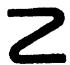
\includegraphics[keepaspectratio]{images/part001_fc188d82.jpg}}

Remark 1. The projection of a closed subset of \(\mathbf{X}_1 \times \mathbf{X}_2\) onto a factor need not be closed. For example, in the rational plane \(\mathbf{Q}^2\) , the hyperbola whose equation is \(x_1 x_2 = 1\) is a closed set, but both its projections are equal to the complement of the point 0 in \(\mathbf{Q}\) , and this is not a closed set.

PROPOSITION 6. Let \(\mathbf{X}_1, \mathbf{X}_2, \mathbf{Y}\) be three topological spaces, \(f\) a mapping of the product space \(\mathbf{X}_1 \times \mathbf{X}_2\) into \(\mathbf{Y}\) . If \(f\) is continuous at the point \((a_1, a_2)\) then the partial mapping \(x_2 \to f(a_1, x_2)\) of \(\mathbf{X}_2\) into \(\mathbf{Y}\) is continuous at the point \(a_2\) .

For this mapping is the composition of \(f\) and the mapping \(x_{2} \to (a_{1}, x_{2})\) ; hence the result follows from Proposition 4.

Proposition 6 is often expressed by saying that a continuous function of two variables is continuous with respect to each of them separately.

\pandocbounded{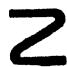
\includegraphics[keepaspectratio]{images/part001_31ca3096.jpg}}

Remark 2. It is possible for all the partial mappings determined by a map \(f: \mathbf{X}_{1} \times \mathbf{X}_{2} \to \mathbf{Y}\) to be continuous without \(f\) being continuous on \(\mathbf{X}_{1} \times \mathbf{X}_{2}\) (cf.~Chapter IX, § 5, Exercise 23). * For example if \(f\) is the mapping of the real plane \(\mathbb{R}^{2}\) into \(\mathbb{R}\) defined by

\[
f (x, y) = x y / \left(x ^ {2} + y ^ {2}\right) \quad \text { if } \quad (x, y) \neq (0, 0)
\]

and \(f(0, 0) = 0\) , then all the partial mappings are continuous; but \(f\) is not continuous at \((0, 0)\) , since \(f(x, x) = 1/2\) if \(x \neq 0\) .

If \(g\) is a mapping of \(\mathbf{X}_1\) into \(\mathbf{Y}\) , continuous at a point \(a_1\) , then the mapping \((x_1, x_2) \to g(x_1)\) of \(\mathbf{X}_1 \times \mathbf{X}_1 \to \mathbf{Y}\) is continuous at all points \((a_1, x_2)\) , for it is the composition of \(g\) and the projection onto \(\mathbf{X}_1\) .

The results of this subsection are easily extended to an arbitrary product \(\prod_{i\in I}X_i\) of topological spaces by remarking that this product is homeomorphic to the product \(\left(\prod_{i\in J}X_i\right)\times\left(\prod_{i\in K}X_i\right)\) for any partition (J, K) of I (no. 1, Proposition 2).

\subsection{CLOSURE IN A PRODUCT}

PROPOSITION 7. In a product space \(\prod_{i\in I}X_i\) , the closure of a product of sets \(\prod_{i\in I}A_i\) is the same as the product \(\prod_{i\in I}\overline{A}_i\) of their closures.

Suppose that \(a = (a_{t})\) lies in the closure of \(\prod_{i} A_{i}\) ; then for each \(x \in I\) , \(a_{x} = \text{pr}_{x} a\) is in the closure of \(A_{x}\) because of the continuity of \(\text{pr}_{x}\) ( \(\S 2\) , no. 1, Theorem 1) and therefore \(a \in \prod_{i} \overline{A}_{i}\) . Conversely, let \(b = (b_{i}) \in \prod_{i} \overline{A}_{i}\) , and let \(\prod_{i} V_{i}\) be any elementary set containing \(b\) ; for each \(i \in I\) , \(V_{i}\) contains a point \(x_{i} \in A_{i}\) ; hence \(\prod_{i} V_{i}\) contains the point \((x_{i}) \in \prod_{i} A_{i}\) and therefore \(b\) lies in the closure of \(\prod A_{i}\) .

COROLLARY. A product \(\prod_{i} A_{i}\) of non-empty sets is closed in the product space \(\prod_{i} X_{i}\) if and only if \(A_{i}\) is closed in \(X_{i}\) for each \(i \in I\) .

If I is finite, a product \(\prod_{i\in I}A_i\) is open provided that \(A_i\) is open in \(X_i\) for each \(i\in I\) ; but this is no longer so if I is infinite.

PROPOSITION 8. Let \(a = (a_{i})\) be any point of a product space \(X = \prod_{i \in I} X_{i}\) ; then the set \(D\) of points \(x \in X\) such that \(\operatorname{pr}_{i} x = a_{i}\) except for a finite number of indices \(i\) is dense in \(X\) .

For each \(x \in \mathbf{X}\) and each elementary set \(V = \prod_{i \in I} U_i\) which contains \(x\) , we have \(U_i = X_i\) except for indices \(i\) belonging to a finite subset \(J\) of \(I\) ; if we take \(y_i = x_i\) for \(i \in J\) and \(y_i = a_i\) for \(i \notin J\) , it is clear that

\[
y = (y _ {i}) \in D \quad \text { and } \quad y \in V;
\]

hence the result.

\subsection{INVERSE LIMITS OF TOPOLOGICAL SPACES}

Let I be a partially ordered (but not necessarily directed) set (*), in which the order relation is written \(\alpha \leqslant \beta\) . For each \(\alpha \in I\) , let \(X_{\alpha}\) be a topological space, and for each pair \((\alpha, \beta)\) such that \(\alpha \leqslant \beta\) let \(f_{\alpha\beta}\) be a mapping of \(X_{\beta}\) into \(X_{\alpha}\) . We say that \((X_{\alpha}, f_{\alpha\beta})\) is an inverse system of topological spaces if: 1) \((X_{\alpha}, f_{\alpha\beta})\) is an inverse system of sets; 2) \(f_{\alpha\beta}\) is a continuous mapping whenever \(\alpha \leqslant \beta\) . Let X denote the set \(\varprojlim X_{\alpha}\) , and for each \(\alpha \in I\) let \(f_{\alpha}\) be the canonical mapping \(X \to X_{\alpha}\) ; then the coarsest topology on X for which the \(f_{\alpha}\) are continuous is said to be the inverse limit (with respect to the \(f_{\alpha\beta}\) ) of the topologies of the \(X_{\alpha}\) , and the set X with this topology is called the inverse limit of the inverse system of topological spaces \((X_{\alpha}, f_{\alpha\beta})\) . Whenever we speak of \(\varprojlim X_{\alpha}\) as a topological space, it is always to be understood that the topology of this space is the inverse limit of the topologies of the \(X_{\alpha}\) , unless the contrary is expressly stated.

The set X is the subset of the product \(\prod_{\alpha\in I}X_{\alpha}\) consisting of those points x such that

\[
\operatorname{pr} _ {\alpha} (x) = f _ {\alpha \beta} (\operatorname{pr} _ {\beta} (x))\tag{I}
\]

whenever \(\alpha \leqslant \beta\) . It follows from Proposition 3 of no. 1 that the inverse limit of the topologies of the \(X_{\alpha}\) is the same as the topology induced on \(X\) by the topology of the product space \(\prod_{\alpha \in I} X_{\alpha}\) . If, for each \(\alpha \in I\) , \(Y_{\alpha}\) is a subspace of \(X_{\alpha}\) such that the \(Y_{\alpha}\) form an inverse system of subsets of the \(X_{\alpha}\) (Set Theory chapter III, § 7, n° 2), then it is clear that the topological space \(\varprojlim Y_{\alpha}\) is a subspace of \(\varprojlim X_{\alpha}\) .

Let \((\mathbf{X}_{\alpha}^{\prime}, f_{\alpha\beta}^{\prime})\) be another inverse system of topological spaces indexed by the same set I, and for each \(\alpha \in I\) let \(u_{\alpha}: X_{\alpha} \to X_{\alpha}^{\prime}\) be a continuous mapping such that \((u_{\alpha})\) is an inverse system of mappings; then \(u = \varprojlim u_{\alpha}\) is a continuous mapping of \(X = \varprojlim X_{\alpha}\) into \(X^{\prime} = \varprojlim X_{\alpha}^{\prime}\) . For if \(f_{\alpha}^{\prime}\) is the canonical mapping \(X^{\prime} \to X_{\alpha}^{\prime}\) , we have \(f_{\alpha}^{\prime} \circ u = u_{\alpha} \circ f_{\alpha}\) , so that \(f_{\alpha}^{\prime} \circ u\) is continuous for each \(\alpha \in I\) , and the assertion follows from Proposition 4 of § 2, no. 3.

Finally, suppose I is a directed set, and let J be a cofinal subset of I; let Z be the inverse limit of the inverse system of topological spaces \((\mathbf{X}_{\alpha}, f_{\alpha\beta})_{\alpha\in\mathbf{J}, \beta\in\mathbf{J}}\) . Then the canonical bijection \(g: X \to Z\) (Set Theory, Chapter III, § 7, no. 2, proposition 3) is a homeomorphism. For we have \(\operatorname{pr}_{\lambda}(g(x)) = \operatorname{pr}_{\lambda}(x)\) for each \(\lambda \in J\) ; hence g is continuous (no. 1, Proposition 1); and if h is the inverse of g, then for each \(\alpha \in I\) there exists \(\lambda \in J\) such that \(\alpha \leqslant \lambda\) , and therefore \(\operatorname{pr}_{\alpha}(h(z)) = f_{\alpha\lambda}(\operatorname{pr}_{\lambda}(z))\) , which shows that h is continuous (no. 1, Proposition 1), since the \(f_{\alpha\lambda}\) are continuous.

PROPOSITION 9. Let I be a directed set and J a cofinal subset of I. Let \((\mathbf{X}_{\alpha}, f_{\alpha \beta})\) be an inverse system of topological spaces indexed by I; let \(\mathbf{X} = \varprojlim \mathbf{X}_{\alpha}\) and let \(f_{\alpha}: \mathbf{X} \to \mathbf{X}_{\alpha}\) be the canonical mapping. Then the family of sets \(\overline{f}_{\alpha}^{1}(\mathbf{U}_{\alpha})\) , where \(\alpha\) runs through J and \(\mathbf{U}_{\alpha}\) runs through a base \(\mathfrak{B}_{\alpha}\) of the topology of \(\mathbf{X}_{\alpha}\) for each \(\alpha \in \mathbf{J}\) , is a base of the topology of \(\mathbf{X}\) .

From § 2, no. 3 we know that the finite intersections of sets of the form \(\overline{f}_{\alpha}^{1}(\mathbf{U}_{\alpha})\) ( \(\alpha \in \mathbf{I}\) , \(\mathbf{U}_{\alpha}\) open in \(\mathbf{X}_{\alpha}\) ) form a base of the topology of \(\mathbf{X}\) . If \((\alpha_i)_{1 \leqslant i \leqslant n}\) is a finite family of indices of \(\mathbf{I}\) , then there exists \(\gamma \in \mathbf{J}\) such that \(\alpha_i \leqslant \gamma\) for \(1 \leqslant i \leqslant n\) ; hence \(f_{\alpha_i} = f_{\alpha_i \gamma} \circ f_\gamma\) ; if we put

\[
\begin{array}{c} \mathrm{V} _ {\gamma} = \bigcap_ {i} \overline {{f}} _ {\alpha_ {i} \gamma} ^ {1} (\mathrm{U} _ {\alpha_ {i}}), \\ \overline {{f}} _ {\gamma} ^ {1} (\mathrm{V} _ {\gamma}) = \bigcap_ {i} \overline {{f}} _ {\alpha_ {i}} ^ {1} (\mathrm{U} _ {\alpha_ {i}}); \end{array}
\]

then we have

but \(V_{\gamma}\) is open and is therefore a union of sets belonging to \(\mathfrak{B}_{\gamma}\) . Hence the result.

COROLLARY. Let A be a subset of X and let \(A_{\alpha}\) denote \(f_{\alpha}(A)\) for each \(\alpha \in I\) . Then:

\begin{enumerate}
\def\labelenumi{(\roman{enumi})}
\item
  The \(\mathbf{A}_{\alpha}\) (resp. the \(\overline{\mathbf{A}}_{\alpha}\) ) form an inverse system of subsets of the \(\mathbf{X}_{\alpha}\) , and \(\overline{\mathbf{A}} = \bigcap_{\alpha} \overline{f}_{\alpha}^{1}(\overline{\mathbf{A}}_{\alpha}) = \varprojlim \overline{\mathbf{A}}_{\alpha}\) .
\item
  If A is closed in X, \(\mathbf{A} = \varprojlim \mathbf{A}_{\alpha} = \varprojlim \overline{\mathbf{A}}_{\alpha}\) .
\end{enumerate}

The first assertion of (i) follows from the relations \(f_{\alpha} = f_{\alpha \beta} \circ f_{\beta}\) for \(\alpha \leqslant \beta\) and from the continuity of the \(f_{\alpha \beta}\) (§ 2, no. 1, Theorem 1). Let \(A'\) denote

\[
\bigcap_ {\alpha} \overline {{f}} _ {\alpha} ^ {1} (\overline {{\mathrm{A}}} _ {\alpha});
\]

then it is clear that \(\mathbf{A}'\) is closed and contains \(\mathbf{A}\) , so that \(\overline{\mathbf{A}} \subset \mathbf{A}'\) . Conversely, let \(x \in \mathbf{A}'\) ; we have to show that \(x\) lies in the closure of \(\mathbf{A}\) . By virtue of Proposition 9 it is enough to prove that every neighbourhood of \(x\) which is of the form \(\overline{f}_{\alpha}^{1}(\mathrm{U}_{\alpha})\) , with \(\alpha \in \mathbf{I}\) and \(\mathbf{U}_{\alpha}\) open in \(\mathbf{X}_{\alpha}\) , meets \(\mathbf{A}\) . Now, by hypothesis, \(f_{\alpha}(x) \in \mathbf{U}_{\alpha}\) , and since \(f_{\alpha}(x) \in \overline{\mathbf{A}}_{\alpha}\) we have \(\mathbf{U}_{\alpha} \cap \mathbf{A}_{\alpha} \neq \emptyset\) , which means that \(\mathbf{A} \cap \overline{f}_{\alpha}^{1}(\mathbf{U}_{\alpha})\) is not empty.

To establish (ii) it is enough to remark that, without any restriction on A, we have \(A \subset \varprojlim A_{\alpha} \subset \varprojlim \overline{A}_{\alpha}\) ; now if A is closed, then from (i)

\[
\mathrm{A} = \varprojlim \overline {{\mathrm{A}}} _ {\alpha}
\]

and (ii) follows.

Example. Let I be a directed set and \((\mathbf{X}_{\alpha})_{\alpha \in I}\) a family of subsets of a set Y, such that \(\mathbf{X}_{\alpha} \supset \mathbf{X}_{\beta}\) whenever \(\alpha \leqslant \beta\) . For each \(\alpha \in I\) let \(\mathfrak{G}_{\alpha}\) be a topology on \(\mathbf{X}_{\alpha}\) such that \(\mathfrak{G}_{\beta}\) is finer than the topology induced on \(\mathbf{X}_{\beta}\) by \(\mathfrak{G}_{\alpha}\) whenever \(\alpha \leqslant \beta\) . If we take \(f_{\alpha \beta}\) to be the canonical injection \(\mathbf{X}_{\beta} \to \mathbf{X}_{\alpha}\) for \(\alpha \leqslant \beta\) , then \(\varprojlim \mathbf{X}_{\alpha}\) may be identified canonically with the intersection X of the \(\mathbf{X}_{\alpha}\) , with the topology which is the least upper bound (§ 2, no. 3, Example 2) of the topologies induced on X by the \(\mathfrak{G}_{\alpha}\) .

\section{OPEN MAPPINGS AND CLOSED MAPPINGS}

\subsection{OPEN MAPPINGS AND CLOSED MAPPINGS}

DEFINITION 1. Let X, X' be two topological spaces. A mapping f: X → X' is open (resp. closed) if the image under f of each open (resp. closed) set of X is open (resp. closed) in X'.

In particular, \(f(\mathbf{X})\) is then an open (resp. closed) subset of \(X'\) .

Examples. 1) Let A be a subspace of a topological space X. Then the canonical injection \(j: \mathbf{A} \to \mathbf{X}\) is open (resp. closed) if and only if A is open (resp. closed) in X ( \(\S\) 3, no. 1).

\begin{enumerate}
\def\labelenumi{\arabic{enumi})}
\setcounter{enumi}{1}
\item
  For a bijection \(f\) of a topological space \(\mathbf{X}\) onto a topological space \(\mathbf{X}'\) to be a homeomorphism it is necessary and sufficient that \(f\) is continuous and open, or continuous and closed.
\item
  Let \(f\) be a surjection of a set \(X\) onto a topological space \(X'\) ; if we give \(X\) the topology which is the inverse image under \(f\) of the topology of \(X'\) (§ 2, no. 3, Example 1), then \(f\) is continuous, open and closed.
\item
  In a product space
\end{enumerate}

\[
\mathbf {X} = \prod_ {i \in \mathbf {I}} \mathbf {X} _ {i},
\]

each projection \(\mathbf{pr}_{t}:\mathbf{X}\to\mathbf{X}_{t}\) is a continuous open mapping, but is not necessarily closed (§ 4, no. 2, Proposition 5).

* 5) A holomorphic function on an open subset A of C is an open mapping of A into C. *

\begin{enumerate}
\def\labelenumi{\arabic{enumi})}
\setcounter{enumi}{5}
\tightlist
\item
  Let X, X' be two topological spaces and f a continuous, but not bicontinuous, bijection of X onto X'. Then the inverse bijection g: \(X' \rightarrow X\) is an open and closed mapping of \(X'\) onto X, but is not continuous.
\end{enumerate}

PROPOSITION 1. Let X, X', X'' be three topological spaces, and let f: X → X', g : X' → X'' be two mappings. Then:

\begin{enumerate}
\def\labelenumi{\alph{enumi})}
\item
  If \(f\) and \(g\) are open (resp. closed), so is \(g \circ f\) .
\item
  If \(g \circ f\) is open (resp. closed) and if \(f\) is continuous and surjective, then \(g\) is open (resp. closed).
\item
  If \(g \circ f\) is open (resp. closed) and if \(g\) is continuous and injective, then \(f\) is open (resp. closed).
\end{enumerate}

From Definition 1. a) follows immediately. To prove b) it is enough to remark that every open (resp. closed) subset \(\mathbf{A}'\) of \(\mathbf{X}'\) can be written as \(f(\mathbf{A})\) , where \(\mathbf{A} = \overline{f}^{1}(\mathbf{A}')\) is open (resp. closed) in \(\mathbf{X}\) ( \(\S 2\) , no. 1, Theorem 1); hence \(g(\mathbf{A}') = g(f(\mathbf{A}))\) is open (resp. closed) in \(\mathbf{X}''\) . Finally, to prove c), we remark that \(f(\mathbf{A}) = \overline{g}^{1}(g(f(\mathbf{A}))\) for every subset \(\mathbf{A}\) of \(\mathbf{X}\) ; by hypothesis, if \(\mathbf{A}\) is open (resp. closed) in \(\mathbf{X}\) , then \(g(f(\mathbf{A}))\) is open (resp. closed) in \(\mathbf{X}''\) , hence \(f(\mathbf{A})\) is open (resp. closed) in \(\mathbf{X}'\) by \(\S 2\) , no. 1, Theorem 1.

PROPOSITION 2. Let X, Y be two topological spaces, f a mapping of X into Y. For each subset T of Y let \(f_{T}\) denote the mapping of \(\overline{f}^{1}(T)\) into T which agrees with f on \(\overline{f}^{1}(T)\) .

\begin{enumerate}
\def\labelenumi{\alph{enumi})}
\item
  If \(f\) is open (resp. closed), \(f_{\mathbf{T}}\) is open (resp. closed).
\item
  Let \((\mathbf{T}(\iota))_{\iota \in \mathbf{I}}\) be a family of subsets of Y whose interiors cover Y, or which is a locally finite closed covering of Y; if all the \(f_{\mathbf{T}(\iota)}\) are open (resp. closed), then \(f\) is open (resp. closed).
\item
  If A is an open (resp. closed) subset of \(\overline{f}^{1}(\mathbf{T})\) , then there is an open (resp. closed) subset B of X such that \(\mathbf{A} = \mathbf{B} \cap \overline{f}^{1}(\mathbf{T})\) , and therefore \(f_{\mathbf{T}}(\mathbf{A}) = f(\mathbf{B}) \cap \mathbf{T}\) ; by hypothesis, \(f(\mathbf{B})\) is open (resp. closed), so that \(f_{\mathbf{T}}(\mathbf{A})\) is open (resp. closed) in \(\mathbf{T}\) .
\item
  Let B be an open (resp. closed) subset of X, and let \(B_{i}\) denote \(\mathbf{B} \cap \overline{f}^{1}(\mathrm{T}(i))\) ; then \(f(\mathbf{B}) \cap \mathrm{T}(i) = f_{\mathbf{T}(i)}(\mathbf{B}_{i})\) . Since \(f_{\mathbf{T}(i)}(\mathbf{B}_{i})\) is open (resp. closed) in \(\mathrm{T}(i)\) by hypothesis, it follows that \(f(\mathbf{B})\) is open (resp. closed) in Y, by Proposition 3 of §3, no. 1.
\end{enumerate}

COROLLARY. Let \((\mathbf{T}(\iota))_{\iota \in \mathbf{I}}\) be a family of subsets of Y whose interiors cover Y, or which is a locally finite closed covering of Y. If \(f: \mathbf{X} \to \mathbf{Y}\) is continuous and if each of the \(f_{\mathbf{T}(\iota)}\) is a homeomorphism of \(\overline{f}^1 (\mathbf{T}(\iota))\) onto \(\mathbf{T}(\iota)\) , then \(f\) is a homeomorphism of \(\mathbf{X}\) onto \(\mathbf{Y}\) .

For \(f\) is clearly bijective, and is open by virtue of Proposition 2.

\subsection{OPEN EQUIVALENCE RELATIONS AND CLOSED EQUIVALENCE RELATIONS}

DEFINITION 2. An equivalence relation R on a topological space X is said to be open (resp. closed) if the canonical mapping of X onto X/R is open (resp. closed).

It comes to the same thing to say that the saturation of each open (resp. closed) subset of X with respect to R is open (resp. closed) in X (§ 3, no. 4).

Examples. 1) Let X be a topological space, \(\Gamma\) a group of homeomorphisms of X onto itself, and let R be the equivalence relation

\[
" \text { there   exists } \sigma \in \Gamma \text { such   that } y = \sigma (x)"
\]

between x and y (thus R is the equivalence relation whose classes are the orbits of \(\Gamma\) in X. The relation R is open, for the saturation of a subset A of X with respect to R is open so is each \(\sigma(\mathbf{A})\) and hence so is their union.

* On the real line R the equivalence relation \(x \equiv y \pmod{1}\) is open, since it is derived as above from the group of translations

\[
x \rightarrow x + n \quad (n \in \mathbf {Z})
\]

(see Chapter III, § 2, no. 4). *

\begin{enumerate}
\def\labelenumi{\arabic{enumi})}
\setcounter{enumi}{1}
\tightlist
\item
  Let X be the sum of a family \((\mathbf{X}_{t})\) of subspaces of X, and let X/R be the space obtained by pasting together the \(X_{t}\) along open subsets \(A_{tx}\) by means of bijections \(h_{xt}\) (§ 2, no. 5); and suppose that \(h_{xt}\) is a homeomorphism of \(A_{tx}\) onto \(A_{xt}\) for each pair of indices \((t, x)\) .
\end{enumerate}

Then the relation R is open. For if U is open in X, the saturation of U is the union of the \(h_{xt}(\mathbf{U} \cap \mathbf{A}_{\mathbf{tx}})\) ; since \(U \cap A_{tx}\) is open in \(A_{tx}\) , \(h_{xt}(\mathbf{U} \cap \mathbf{A}_{\mathbf{tx}})\) is open in \(A_{xt}\) and therefore in X.

\begin{enumerate}
\def\labelenumi{\arabic{enumi})}
\setcounter{enumi}{2}
\tightlist
\item
  With the notation of Example 2, suppose now that the \(\mathbf{A}_{\mathrm{tx}}\) are closed and the \(h_{xt}\) are homeomorphisms; further suppose that for each index \(t\) there is only a finite number of indices \(x\) such that \(\mathbf{A}_{\mathrm{tx}} \neq \emptyset\) (i.e.~each \(\mathbf{X}_t\) is ``stuck'' to only a finite number of \(\mathbf{X}_x\) ). Then the relation R is closed. For if F is any closed subset of X, the saturation of F is the union of the sets \(h_{xt}(\mathbf{F} \cap \mathbf{A}_{\mathrm{tx}}) \subset \mathbf{A}_{xt}\) ; the assumptions made imply that this family is locally finite, and \(h_{xt}(\mathbf{F} \cap \mathbf{A}_{\mathrm{tx}})\) is closed in \(\mathbf{A}_{xt}\) and therefore in X. The result therefore follows from Proposition 4 of § 2, no. 5.
\end{enumerate}

PROPOSITION 3. Let X, Y be two topological spaces, let \(f: \mathbf{X} \to \mathbf{Y}\) be a continuous mapping, let R be the equivalence relation \(f(x) = f(y)\) on X, and let \(\mathbf{X} \xrightarrow{p} \mathbf{X}/\mathbf{R} \xrightarrow{h} f(\mathbf{X}) \xrightarrow{i} \mathbf{Y}\) be the canonical decomposition of \(f\) . Then the following three statements are equivalent:

\begin{enumerate}
\def\labelenumi{\alph{enumi})}
\item
  \(f\) is an open mapping.
\item
  The three mappings \(p, h, i\) are open.
\item
  The equivalence relation R is open, h is a homeomorphism, and \(f(\mathbf{X})\) is an open subset of Y.
\end{enumerate}

Also the preceding proposition remains true if ``open'' is replaced by ``closed'' throughout.

Since the injection \(i\) is continuous, it follows from Proposition 1c) of no. 1 that if \(f\) is open then so is \(h \circ p\) ; since \(p\) is surjective and continuous, Proposition 1b) shows that \(h\) is open; \(h\) is in any case a continuous bijection; thus \(h\) is a homeomorphism, and therefore, from Proposition 1a) of no. 1, \(p = \overline{h}^1 \circ (h \circ p)\) is an open mapping. Also {[}no. 1, Proposition 1b){]} \(i \circ h\) is open; hence {[}no. 1, Proposition 1a){]} so is \(i = (i \circ h) \circ \overline{h}^1\) . This proves that a) implies b). Conversely, Proposition 1a) of no. 1 shows that b) implies a). Finally, the equivalence of b) and c) follows immediately from the definitions.

The proof in the case of closed mappings is analogous, mutatis mutandis.

PROPOSITION 4. Let R be an open (resp. closed) equivalence relation on a topological space X, and f the canonical mapping X → X/R. Let A be a subset of X and suppose that one of the following two conditions is satisfied: a) A is open (resp. closed) in X.

\begin{enumerate}
\def\labelenumi{\alph{enumi})}
\setcounter{enumi}{1}
\tightlist
\item
  A is saturated with respect to R.
\end{enumerate}

Then the relation \(R_{A}\) induced on A is open (resp. closed) and the canonical mapping of \(A/R_{A}\) onto \(f(A)\) is a homeomorphism.

Consider the commutative diagram (1) of § 3, no. 6, which gives the canonical decomposition of \(f \circ j\) . Under condition a), \(j\) is open (resp. closed) and so is \(f\) by hypothesis; hence \(f \circ j\) is open (resp. closed) {[}no. 1, Proposition 1 a){]}, and the result follows from Proposition 3. Under condition b) we have

\[
\mathbf {A} = \overline {{{f}}} ^ {1} (f (\mathbf {A})),
\]

and \(h \circ \varphi\) is the mapping of A into \(f(A)\) which agrees with \(f\) on A; by virtue of Proposition 2 a) of no. 1, \(h \circ \varphi\) is open (resp. closed), and the result again follows from Proposition 3, applied to \(h \circ \varphi\) .

\subsection{PROPERTIES PECULIAR TO OPEN MAPPINGS}

PROPOSITION 5. Let X, Y be two topological spaces, f a mapping of X into Y, B a base of the topology of X. Then the following statements are equivalent:

\begin{enumerate}
\def\labelenumi{\alph{enumi})}
\item
  \(f\) is an open mapping.
\item
  For each \(\mathbf{U} \in \mathfrak{B}\) , \(f(\mathbf{U})\) is open in \(\mathbf{Y}\) .
\item
  For each \(x \in \mathbf{X}\) and each neighbourhood \(\mathbf{V}\) of \(x\) in \(\mathbf{X}\) , \(f(\mathbf{V})\) is a neighbourhood of \(f(x)\) in \(\mathbf{Y}\) .
\end{enumerate}

The equivalence of a) and b) follows immediately from the definitions and from \((\mathrm{O}_{\mathrm{I}})\) ; the equivalence of a) and c) is a consequence of Proposition 1 of §1, no. 2.

PROPOSITION 6. Let R be an equivalence relation on a topological space X; then the following three conditions are equivalent:

\begin{enumerate}
\def\labelenumi{\alph{enumi})}
\item
  The relation \(\mathbf{R}\) is open.
\item
  The interior of each subset which is saturated with respect to R is saturated with respect to R.
\item
  The closure of each subset which is saturated with respect to R is saturated with respect to R.
\end{enumerate}

By taking complements (§ 1, no. 6, formula (2)) we see that b) and c) are equivalent. Let us show that b) implies a): suppose condition b) is satisfied and let U be an open subset of X, V its saturation with respect to R; then \(\dot{V} \supset U\) , and since by hypothesis \(\dot{V}\) is saturated, it follows that \(\dot{V} = V\) , and therefore the saturation of U is open. Conversely, suppose condition a) is satisfied, and let A be a saturated set; if B is the saturation of \(\mathring{A}\) , then \(\mathring{A} \subset B \subset A\) , and since B is open by hypothesis it follows that \(B = \mathring{A}\) .

PROPOSITION 7. Let R be an open equivalence relation on a topological space X, and let \(\varphi: \mathbf{X} \to \mathbf{X}/\mathbf{R}\) be the canonical mapping. If A is any subset of X which is saturated with respect to R, then the closure (resp. the interior) of \(\varphi(\mathbf{A})\) in X/R is \(\varphi(\overline{\mathbf{A}})\) (resp. \(\varphi(\mathring{\mathbf{A}})\) ).

Each of the two assertions of the proposition can be deduced from the other by taking complements and using formula (2) of § 1, no. 6 and the fact that if B is a saturated subset of X then \(\varphi(\complement B) = \complement \varphi(B)\) . By virtue of Proposition 6, \(\overline{A}\) is saturated; hence \(\varphi(\overline{A})\) is closed in \(X/R\) , and since \(A \subset \overline{A}\) we have \(\overline{\varphi(A)} \subset \varphi(\overline{A})\) , so that \(\varphi(A) \subset \varphi(\overline{A})\) . But since \(\varphi\) is continuous, \(\varphi(\overline{A}) \subset \overline{\varphi(A)}\) ( \(\S 2\) , no. 1, Theorem 1), and the result follows.

PROPOSITION 8. Let \((\mathbf{X}_t)_{t \in \mathbf{I}}\) , \((\mathbf{Y}_t)_{t \in \mathbf{I}}\) be two families of topological spaces indexed by the same set I. For each \(t \in \mathbf{I}\) let \(f_t\) be an open mapping of \(\mathbf{X}_t\) into \(\mathbf{Y}_t\) , and suppose that \(f_t\) is surjective for all but a finite number of indices. Then the product mapping \(f: (x_t) \to (f_t(x_t))\) of \(\prod_{t \in \mathbf{I}} \mathbf{X}_t\) into \(\prod_{t \in \mathbf{I}} \mathbf{Y}_t\) is open.

By virtue of Proposition 5 we need only prove that the image under \(f\) of any elementary set \(\prod_{t \in I} A_t\) in \(\prod_{t \in I} X_t\) is open in \(\prod_{t \in I} Y_t\) . But this image is \(\prod_{t \in I} f_t(A_t)\) , and the hypotheses imply that \(f_t(A_t)\) is open in \(Y_t\) for each \(t \in I\) , and that \(f_t(A_t) = Y_t\) for all but a finite number of indices; whence the result.

COROLLARY. Let \((\mathbf{X}_t)_{t \in I}\) be a family of topological spaces, and for each \(t \in I\) let \(\mathbf{R}_t\) be an equivalence relation on \(\mathbf{X}_t\) , and let \(f_t\) be the canonical mapping \(\mathbf{X}_t \to \mathbf{X}_t / \mathbf{R}_t\) . Let \(\mathbf{R}\) be the equivalence relation in \(\mathbf{X} = \prod_{t \in I} \mathbf{X}_t\) ``for each \(t \in I\) , \(\operatorname{pr}_t(x) = \operatorname{pr}_t(y) (\bmod \mathbf{R}_t)"\)

between \(x\) and \(y\) , and let \(f\) be the product mapping \((x_{t}) \to (f_{t}(x_{t}))\) of \(X\) into \(\prod_{t \in I} (X_{t}/R_{t})\) . If each of the relations \(R_{t}\) is open, then the relation \(R\) is open, and the bijection associated with \(f\) is a homeomorphism of \(X/R\) onto \(\prod_{t \in I} (X_{t}/R_{t})\) .

R is the relation \(f(x)=f(y)\) . Since f is continuous and open by Proposition 8 above and § 4, no. 1, Corollary 1 of Proposition 1, the result follows from Proposition 3 of no. 2.

In particular, if R (resp. S) is an open equivalence relation on a topological space X (resp. Y), then the canonical bijection of

\[
(\mathbf {X} \times \mathbf {Y}) / (\mathbf {R} \times \mathbf {S}) \quad \text { onto } \quad (\mathbf {X} / \mathbf {R}) \times (\mathbf {Y} / \mathbf {S})
\]

\pandocbounded{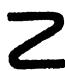
\includegraphics[keepaspectratio]{images/part001_bebaa45c.jpg}}

is a homeomorphism. If R and S are not assumed to be open, this bijection is continuous but is not necessarily a homeomorphism, even if one of the relations R, S is the relation of equality (Exercise 6).

\subsection{PROPERTIES PECULIAR TO CLOSED MAPPINGS}

PROPOSITION 9. Let X, X' be two topological spaces. A necessary and sufficient condition for a mapping \(f: \mathbf{X} \to \mathbf{X}'\) to be continuous and closed is that \(f(\overline{\mathbf{A}}) = \overline{f(\mathbf{A})}\) for every subset A of X.

The condition is sufficient, for it obviously implies that \(f\) is closed, and it also implies that \(f\) is continuous by reason of § 2, no. 1, Theorem 1. Conversely, if \(f\) is continuous and closed, we have \(f(\mathbf{A}) \subset f(\overline{\mathbf{A}}) \subset \overline{f(\mathbf{A})}\) by § 2, no. 1, Theorem 1; also \(f(\overline{\mathbf{A}})\) is closed in \(\mathbf{X}'\) by hypothesis; hence \(f(\overline{\mathbf{A}}) = \overline{f(\mathbf{A})}\) .

PROPOSITION 10. Let R be an equivalence relation on a topological space X. Then R is closed if and only if every equivalence class M mod R possesses a fundamental system of neighbourhoods which are saturated with respect to R.

Suppose R is closed, and let U be an arbitrary open neighbourhood of M; since \(F = \complement U\) is closed in X, the saturation S of F with respect to R is closed in X. Since M is saturated with respect to R, we have \(M \cap S = \varnothing\) , and thus \(V = \complement S\) is an open neighbourhood of M, saturated with respect to R and contained in U.

To prove the converse, let F be any closed subset of X. Let T be the saturation of F with respect to R, let x be a point of \(\complement T\), and let M be the equivalence class of x; then \(M \cap T = \varnothing\) and a fortiori \(M \cap F = \varnothing\) , so that U = \(\complement F\) is a neighbourhood of M. Hence there is a neighbourhood \(V \subset U\) of M such that V is saturated with respect to R; V does not meet F, hence does not meet T, so that \(\complement T\) is a neighbourhood of M and therefore of x. This shows that \(\complement T\) is open (§ 1, no. 2, Proposition 1), i.e.~T is closed.

Remark. Proposition 10 implies the following: if R is closed and if \(\varphi\) denotes the canonical mapping \(X \to X/R\) , then for each \(x \in X\) and each neighbourhood U of the equivalence class of \(x\) in X, \(\varphi(U)\) is a neighbourhood of \(\varphi(x)\) in X/R. It should be carefully noticed that this statement by no means implies that for every neighbourhood V of \(x\) , \(\varphi(V)\) is a neighbourhood of \(\varphi(x)\) ; in other words (no. 3, Proposition 5) a closed equivalence relation is not necessarily open (Exercise 2). Conversely, an open equivalence relation is not necessarily closed (no. 1, Example 4);

\pandocbounded{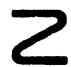
\includegraphics[keepaspectratio]{images/part001_bfecd507.jpg}}

for if U is a neighbourhood in X of an equivalence class M, then for each \(x \in M\) and each neighbourhood \(V \subset U\) of x, the saturation of V is certainly a neighbourhood of M in X, but this neighbourhood is not necessarily contained in U.

Finally, there are equivalence relations other than equality which are both open and closed (Exercise 3) and equivalence relations which are neither open nor closed ( \(§\ 8\) , Exercise 10).

\section{FILTERS}

\subsection{DEFINITION OF A FILTER}

DEFINITION 1. A filter on a set X is a set F of subsets of X which has the following properties:

(F \(_{I}\) ) Every subset of X which contains a set of F belongs to F.

\((\mathbf{F}_{\mathrm{II}})\) Every finite intersection of sets of \(\mathfrak{F}\) belongs to \(\mathfrak{F}\) .

\((\mathbf{F}_{\mathrm{III}})\) The empty set is not in \(\mathfrak{F}\) .

It follows from \((\mathbf{F}_{\mathbf{II}})\) and \((\mathbf{F}_{\mathbf{III}})\) that every finite intersection of sets of F is non-empty.

A filter \(\mathfrak{F}\) on X defines a structure on X, the axioms of which are \((\mathrm{F_I})\) , \((\mathrm{F_{II}})\) and \((\mathrm{F_{III}})\) ; this structure is called a structure of a filtered set, and the set X endowed with this structure is called a set filtered by \(\mathfrak{F}\) .

Axiom \((\mathbf{F}_{\mathrm{II}})\) is equivalent to the conjunction of the following two axioms: \((\mathbf{F}_{\mathrm{II}a})\) The intersection of two sets of F belongs to F.

\((\mathbf{F}_{\mathrm{II}b})\) X belongs to \(\mathfrak{F}\) .

Axioms \((\mathbf{F}_{\mathbf{II}\ \mathbf{b}})\) and \((\mathbf{F}_{\mathbf{III}})\) show that there is no filter on the empty set.

In order for a set of subsets which satisfies \((\mathbf{F}_{\mathbf{I}})\) also to satisfy \((\mathbf{F}_{\mathbf{II}\mathbf{b}})\) it is necessary and sufficient that it is not empty. A set of subsets which satisfies \((\mathbf{F}_{\mathbf{I}})\) also satisfies \((\mathbf{F}_{\mathbf{III}})\) if and only if it is different from \(\mathfrak{P}(\mathbf{X})\) .

Examples of filters. 1) If \(\mathbf{X} \neq \emptyset\) , the set of subsets consisting of \(\mathbf{X}\) alone is a filter on \(\mathbf{X}\) . More generally, the set of all subsets of \(\mathbf{X}\) which contain a given non-empty subset \(\mathbf{A}\) of \(\mathbf{X}\) is a filter on \(\mathbf{X}\) .

\begin{enumerate}
\def\labelenumi{\arabic{enumi})}
\setcounter{enumi}{1}
\item
  In a topological space X, the set of all neighbourhoods of an arbitrary non-empty subset A of X (and in particular the set of all neighbourhoods of a point of X) is a filter, called the neighbourhood filter of A.
\item
  If X is an infinite set, the complements of the finite subsets of X are the elements of a filter. The filter of complements of finite subsets of the set N of integers \(\geqslant0\) is called the Fréchet filter.
\end{enumerate}

\subsection{COMPARISON OF FILTERS}

DEFINITION 2. Given two filters \(\mathfrak{F}\) , \(\mathfrak{F}'\) on the same set X, \(\mathfrak{F}'\) is said to be finer than \(\mathfrak{F}\) , or \(\mathfrak{F}\) is coarser than \(\mathfrak{F}'\) , if \(\mathfrak{F} \subset \mathfrak{F}'\) . If also \(\mathfrak{F} \neq \mathfrak{F}'\) , then \(\mathfrak{F}'\) is said to be strictly finer than \(\mathfrak{F}\) , or \(\mathfrak{F}\) strictly coarser than \(\mathfrak{F}'\) .

Two filters are said to be comparable if one is finer than the other. The set of all filters on X is ordered by the relation ``F is coarser than F''; this relation is induced by the inclusion relation in \(\mathfrak{P}(\mathfrak{P}(\mathbf{X}))\) .

Let \((\mathfrak{F}_t)_{\iota \in I}\) be any non-empty family of filters on a set \(X\) (which must therefore be non-empty); then the set

\[
\mathfrak {F} = \bigcap_ {i \in I} \mathfrak {F} _ {i}
\]

satisfies axioms \((\mathbf{F}_{\mathbf{I}})\) , \((\mathbf{F}_{\mathbf{II}})\) and \((\mathbf{F}_{\mathbf{III}})\) and is therefore a filter; F is called the intersection of the family of filters \((\mathfrak{F}_{i})_{i\in\mathbf{I}}\) and is obviously the greatest lower bound of the set of the \(F_{i}\) in the ordered set of all filters on X.

The filter formed by the single set X is the smallest element of the ordered set of all filters on X. We shall see in no. 4 that, if X has more than one element, the set of all filters on X has no greatest element.

Given a set \(\mathfrak{G}\) of subsets of a set X, let us consider whether there are any filters on X which contain \(\mathfrak{G}\) . If such a filter exists then by \((\mathrm{F}_{\mathrm{II}})\) it contains also the set \(\mathfrak{G}'\) of finite intersections of sets of \(\mathfrak{G}\) (including X, which is the intersection of the empty subset of \(\mathfrak{G}\) ); hence a necessary condition for such a filter to exist is that the empty subset of X is not in \(\mathfrak{G}'\) . This condition is also sufficient, for by \((\mathrm{F}_{\mathrm{I}})\) any filter which contains \(\mathfrak{G}'\) also contains the set \(\mathfrak{G}''\) of subsets of X which contain a set of \(\mathfrak{G}'\) . Now \(\mathfrak{G}''\) clearly satisfies \((\mathrm{F}_{\mathrm{I}})\) ; it satisfies \((\mathrm{F}_{\mathrm{II}})\) by reason of the definition of \(\mathfrak{G}'\) ; and finally it satisfies \((\mathrm{F}_{\mathrm{III}})\) because the empty subset of X does not belong to \(\mathfrak{G}'\) . Hence \(\mathfrak{G}''\) is the coarsest filter which contains \(\mathfrak{G}\) , and we have proved:

PROPOSITION 1. A necessary and sufficient condition that there should exist a filter on X containing a set \(\mathfrak{G}\) of subsets of X is that no finite subset of \(\mathfrak{G}\) has an empty intersection.

The filter \(\mathfrak{G}''\) defined above is said to be generated by \(\mathfrak{G}\) , and \(\mathfrak{G}\) is said to be a subbase of \(\mathfrak{G}''\) .

Example. Let \(\mathfrak{S}\) be any set of subsets of a set X, and let \(\mathfrak{C}\) be the topology on X generated by \(\mathfrak{S}\) ( \(\S\) 2, no. 3, Example II). Since the set of finite intersections of sets of \(\mathfrak{S}\) is a base of \(\mathfrak{C}\) , it follows from the proof of Proposition 1 above and from Proposition 3 of \(\S\) 1, no. 3 that for each \(x \in X\) the neighbourhood filter of \(x\) for \(\mathcal{C}\) is generated by the set \(\mathfrak{S}(x)\) of sets of \(\mathfrak{S}\) which contain \(x\) .

COROLLARY 1. Let \(\mathfrak{F}\) be a filter on a set X, and A a subset of X. Then there is a filter \(\mathfrak{F}'\) which is finer than \(\mathfrak{F}\) and such that \(A \in \mathfrak{F}'\) , if and only if A meets all the sets of \(\mathfrak{F}\) .

COROLLARY 2. A set \(\Phi\) of filters on a non-empty set \(\mathbf{X}\) has a least upper bound in the set of all filters on \(\mathbf{X}\) if and only if, for all finite sequences \((\mathfrak{F}_i)_{1\leqslant i\leqslant n}\) of elements of \(\Phi\) and all \(\mathrm{A}_i\in \mathfrak{F}_i\) ( \(1\leqslant i\leqslant n\) ), the intersection \(\mathrm{A}_1\cap \dots \cap \mathrm{A}_n\) is not empty.

For this condition expresses that the union \(\mathfrak{G}\) of the filters \(\mathfrak{F} \in \Phi\) satisfies the condition of Proposition 1.

COROLLARY 3. The ordered set of all filters on a non-empty set X is inductive.

For every linearly ordered set \(\Phi\) of filters on \(X\) satisfies the condition of Corollary 2 of Proposition 1, since the sets \(A_{i}\) all belong to the same \(\mathfrak{F}_{j}\) by hypothesis, and we can apply \((\mathbf{F}_{\mathrm{II}})\) .

\subsection{BASES OF A FILTER}

If \(\mathfrak{G}\) is a subbase of a filter \(\mathfrak{F}\) on X (no. 2), then \(\mathfrak{F}\) is not in general the set of subsets of X which contain a set of \(\mathfrak{G}\) ; for \(\mathfrak{G}\) to have this property it is necessary and sufficient that every finite intersection of sets of \(\mathfrak{G}\) should contain a set of \(\mathfrak{G}\) . Hence the following proposition:

PROPOSITION 2. Let \(\mathfrak{B}\) be a set of subsets of a set X. Then the set of subsets of X which contain a set of \(\mathfrak{B}\) is a filter if and only if \(\mathfrak{B}\) has the following two properties:

(B \(_{I}\) ) The intersection of two sets of B contains a set of B.

(B \(_{II}\) ) B is not empty, and the empty subset of X is not in B.

DEFINITION 3. A set B of subsets of a set X which satisfies axioms (B \(_{I}\) ) and (B \(_{II}\) ) is said to be a base of the filter it generates. Two filter bases are said to be equivalent if they generate the same filter.

If \(\mathfrak{G}\) is a subbase of a filter \(\mathfrak{F}\) , then the set \(\mathfrak{G}'\) of finite intersections of sets of \(\mathfrak{G}\) is a base of \(\mathfrak{F}\) (no. 2).

PROPOSITION 3. A subset \(\mathfrak{B}\) of a filter \(\mathfrak{F}\) on \(\mathbf{X}\) is a base of \(\mathfrak{F}\) if and only if every set of \(\mathfrak{F}\) contains a set of \(\mathfrak{B}\) .

If \(\mathfrak{B}\) is a base of \(\mathfrak{F}\) , then clearly every set of \(\mathfrak{F}\) contains a set of \(\mathfrak{B}\) ; conversely, if every set of \(\mathfrak{F}\) contains a set of \(\mathfrak{B}\) , then the set of subsets of \(X\) containing a set of \(\mathfrak{B}\) coincides with \(\mathfrak{F}\) by reason of \((\mathbf{F}_{\mathbf{I}})\) .

For example, the Fréchet filter (no. 1) is the section filter of the ordered set N, considered as directed by the relation \(\leqslant\). Let \(\mathfrak{F}\) be a filter on a set Z. Since \(\mathfrak{F}\) is directed with respect to the relation \(\supset\) {[}by reason of axiom \((\mathrm{F}_{\mathrm{II}})\){]} we can define a section filter on \(\mathfrak{F}\); here a section of \(\mathfrak{F}\) relative to a set A\(\in\mathfrak{F}\) is the set S(A) of all M\(\in\mathfrak{F}\) such that M\(\subset\)A. This filter is called the section filter of the filter \(\mathfrak{F}\).

PROPOSITION 4. On a set X, a filter \(\mathfrak{F}'\) with base \(\mathfrak{B}'\) is finer than a filter \(\mathfrak{F}\) with base \(\mathfrak{B}\) if and only if every set of \(\mathfrak{B}\) contains a set of \(\mathfrak{B}'\) .

This is an immediate consequence of Definitions 2 and 3.

COROLLARY. Two filter bases B, B' on a set X are equivalent if and only if every set of B contains a set of B' and every set of B' contains a set of B.

Examples of filter bases. 1) Let X be a topological space. Proposition 3 shows that the bases of the neighbourhood filter of a point \(x \in X\) are precisely the fundamental systems of neighbourhoods of \(x\) (§ 1, no. 3, Definition 5).

\begin{enumerate}
\def\labelenumi{\arabic{enumi})}
\setcounter{enumi}{1}
\tightlist
\item
  Let X be a non-empty directed set with respect to a relation \((\sigma)\) (Set Theory, Chapter III, § 1, no. 10). For each \(a \in X\) , the set \(S(a)\) of all \(x \in X\) such that \(a(\sigma)x\) will be called the section of X relative to the element a. Then the set S of sections of X is a filter base, for it clearly satisfies \((\mathbf{B}_{\mathbf{II}})\) , and if a, b are any two elements of X, then there is by hypothesis an element \(c \in X\) such that \(a(\sigma)c\) and \(b(\sigma)c\) , and therefore
\end{enumerate}

\[
\mathbf {S} (c) \subset \mathbf {S} (a) \cap \mathbf {S} (b),
\]

so that \((\mathbf{B}_{\mathbf{I}})\) is satisfied. The filter generated by S is called the section filter of the directed set X.

\subsection{ULTRAFILTERS}

DEFINITION 4. An ultrafilter on a set X is a filter F such that there is no filter on X which is strictly finer than F (in other words, a maximal element in the ordered set of all filters on X).

Since the ordered set of all filters on X is inductive (no. 2, Proposition 1, Corollary 3), Zorn's lemma (Set Theory, R, § 6, no. 10) shows that:

THEOREM 1. If F is any filter on a set X, there is an ultrafilter finer than F.

PROPOSITION 5. Let \(\mathfrak{F}\) be an ultrafilter on a set \(\mathbf{X}\) . If \(\mathbf{A}\) and \(\mathbf{B}\) are two subsets of \(\mathbf{X}\) such that \(\mathbf{A} \cup \mathbf{B} \in \mathfrak{F}\) , then either \(\mathbf{A} \in \mathfrak{F}\) or \(\mathbf{B} \in \mathfrak{F}\) .

If the proposition is false, there exist subsets A and B of X such that A∉F and B∉F and A∪B∈F. Let G be the set of subsets M of X such that A∪M∈F. It is straightforward to check that G is a filter on X, and G is strictly finer than F, since B∈G; but this contradicts the hypothesis that F is an ultrafilter.

COROLLARY. If the union of a finite sequence \((\mathbf{A}_i)_{1 \leqslant i \leqslant n}\) of subsets of \(\mathbf{X}\) belongs to an ultrafilter \(\mathfrak{F}\) , then at least one of the \(\mathbf{A}_i\) belongs to \(\mathfrak{F}\) .

Proof is by induction on n.

In particular, if \((\mathbf{A}_i)_{1\leqslant i\leqslant n}\) is a covering of \(\mathbf{X}\) , then at least one of the \(\mathbf{A}_i\) belongs to \(\mathfrak{F}\) .

Proposition 5 characterizes the ultrafilters; more generally, we have:

PROPOSITION 6. Let \(\mathfrak{G}\) be a subbase of a filter on a set X. If for each subset Y of X we have either \(Y \in \mathfrak{G}\) or \(\complement Y \in \mathfrak{G}\) , then \(\mathfrak{G}\) is an ultrafilter on X.

Let \(\mathfrak{F}\) be a filter containing \(\mathfrak{G}\) (there is one, by hypothesis); then \(\mathfrak{F}\) coincides with \(\mathfrak{G}\) ; for if \(Y \in \mathfrak{F}\) then \(\complement Y \notin \mathfrak{F}\) ; hence \(\complement Y \notin \mathfrak{G}\) and therefore \(Y \in \mathfrak{G}\) .

Example of an ultrafilter. The set of all subsets of a non-empty set X which contain a given element \(a \in X\) is an ultrafilter; for it is a filter, and if Y is any subset of X then either \(a \in Y\) or \(a \in \complement Y\) . Such ultrafilters are called trivial.

Apart from this example, we shall never prove the existence of an ultrafilter (even on a countably infinite set) except by using Theorem 1 (and therefore the axiom of choice).

Remark. If X contains at least two elements, there are at least two distinct ultrafilters on X, and therefore the ordered set of filters on X has no greatest element.

PROPOSITION 7. Every filter \(\mathfrak{F}\) on a set \(X\) is the intersection of the ultrafilters finer than \(\mathfrak{F}\) .

Clearly this intersection contains \(\mathfrak{F}\) . Conversely, let \(A\) be a subset of \(X\) which does not belong to \(\mathfrak{F}\) , and let \(A'\) denote \(\complement A\) ; \(A\) contains no set of \(\mathfrak{F}\) ; hence every \(M \in \mathfrak{F}\) meets \(A'\) and therefore (no. 2, Proposition 1, Corollary 1) there is a filter \(\mathfrak{F}'\) which is finer than \(\mathfrak{F}\) and contains \(A'\) . If \(\mathfrak{U}\) is an ultrafilter finer than \(\mathfrak{F}'\) (Theorem 1) it follows that \(A \notin \mathfrak{U}\) . This completes the proof.

\subsection{INDUCED FILTER}

PROPOSITION 8. Let \(\mathfrak{F}\) be a filter on a set X and A a subset of X. Then the trace \(\mathfrak{F}_{\mathrm{A}}\) of \(\mathfrak{F}\) on A is a filter if and only if each set of \(\mathfrak{F}\) meets A.

Since \((\mathbf{M} \cap \mathbf{N}) \cap \mathbf{A} = (\mathbf{M} \cap \mathbf{A}) \cap (\mathbf{N} \cap \mathbf{A})\) we see that \(\mathfrak{F}_{\mathbf{A}}\) satisfies \((\mathbf{F}_{\mathbf{II}})\) ; again, if \(\mathbf{M} \cap \mathbf{A} \subset \mathbf{P} \subset \mathbf{A}\) then \(\mathbf{P} = (\mathbf{M} \cup \mathbf{P}) \cap \mathbf{A}\) , whence \(\mathfrak{F}_{\mathbf{A}}\) satisfies \((\mathbf{F}_{\mathbf{I}})\) . Hence \(\mathfrak{F}_{\mathbf{A}}\) is a filter if and only if it satisfies \((\mathbf{F}_{\mathbf{III}})\) , i.e.~if and only if each set of \(\mathfrak{F}\) meets \(\mathbf{A}\) .

In particular, if \(\mathbf{A} \in \mathfrak{F}\) then \(\mathfrak{F}_{\mathbf{A}}\) is a filter on \(\mathbf{A}\) , by \((\mathbf{F}_{\mathbf{II}})\) and \((\mathbf{F}_{\mathbf{III}})\) .

DEFINITION 5. Let A be a subset of a set X and F a filter on X. If the trace of F on A is a filter on A, this filter is said to be induced by F on A.

If a filter \(\mathfrak{F}\) on \(X\) induces a filter on \(A \subset X\) , then the trace on \(A\) of a base of \(\mathfrak{F}\) is a base of \(\mathfrak{F}_A\) , by reason of Proposition 3 of no. 3.

Example. Let X be a topological space, A a subset of X, x a point of X. In order that the trace on A of the neighbourhood filter B of x should be a filter on A, it is necessary and sufficient that every neighbourhood of x meets A, i.e.~that x lies in the closure of A (§ 1, no. 6, Definition 10).

This example of an induced filter is of interest for two reasons: first because it plays an important role in the theory of limits (§ 7, no. 5) and secondly because every filter can be defined in this way. Indeed, let F be a filter on a set X and let X' be the set obtained by adjoining a new element ω to X, X being identified with the complement of \{ω\} in X' (Set Theory, R, § 4, no. 5); let F' be the filter on X' consisting of the sets M ∪ \{ω\} where M runs through F. For each point x ≠ ω of X', let B(x) be the set of all subsets of X' which contain x, and let B(ω) be F'; then the B(x) for x ∈ X' obviously satisfy axioms (V₁), (V₂), (V₃) and (V₄) and therefore define a topology on X' for which they are the neighbourhood filters of points. Finally ω lies in the closure of X in this topology, and F is induced by F' = B(ω) on X. The topology thus defined on X' (resp. the set X' with this topology) is called the topology (resp. the topological space) associated with F.

PROPOSITION 9. An ultrafilter \(\mathfrak{U}\) on a set \(X\) induces a filter on a subset \(A\) of \(X\) if and only if \(A \in \mathfrak{U}\) ; and if this condition is satisfied then \(\mathfrak{U}_A\) is an ultrafilter on \(A\) .

This is an immediate consequence of Propositions 5 and 6 of no. 4.

\subsection{DIRECT IMAGE AND INVERSE IMAGE OF A FILTER BASE}

Let \(\mathfrak{B}\) be a filter base on a set \(\mathbf{X}\) , and let \(f\) be a mapping of \(\mathbf{X}\) into a set \(\mathbf{X}'\) ; then \(f(\mathfrak{B})\) is a filter base on \(\mathbf{X}'\) , for the relation \(\mathbf{M} \neq \emptyset\) implies \(f(\mathbf{M}) \neq \emptyset\) , and we have \(f(\mathbf{M} \cap \mathbf{N}) \subset f(\mathbf{M}) \cap f(\mathbf{N})\) . If \(\mathfrak{B}_1\) is a base of a filter which is finer than the filter of base \(\mathfrak{B}\) , then \(f(\mathfrak{B}_1)\) is a base of a filter finer than the filter of base \(f(\mathfrak{B})\) (no. 3, Proposition 4).

PROPOSITION 10. If \(\mathfrak{B}\) is an ultrafilter base on a set X and if \(f\) is a mapping of X into a set \(\mathbf{X}'\) , then \(f(\mathfrak{B})\) is an ultrafilter base on \(\mathbf{X}'\) .

Let \(\mathbf{M}'\) be a subset of \(\mathbf{X}'\) . If \(\overline{f}^{1}(\mathbf{M}')\) contains a set \(\mathbf{M}\) of \(\mathfrak{B}\) , then \(\mathbf{M}'\) contains \(f(\mathbf{M})\) ; if not, then \(\complement \overline{f}^{1}(\mathbf{M}') = \overline{f}^{1}(\complement \mathbf{M}')\) contains a set \(\mathbf{N}\) of \(\mathfrak{B}\) (no. 4, Proposition 5) and therefore \(\complement \mathbf{M}'\) contains \(f(\mathbf{N})\) . Hence the result follows from Proposition 6 of no. 4.

Consider in particular the case where \(f\) is the canonical injection \(\mathbf{A} \to \mathbf{X}\) of a subset \(\mathbf{A}\) of a set \(\mathbf{X}\) . If \(\mathfrak{B}\) is a filter base on \(\mathbf{A}\) then \(f(\mathfrak{B})\) is a filter base on \(\mathbf{X}\) . The filter \(\mathfrak{F}\) on \(\mathbf{X}\) generated by \(f(\mathfrak{B})\) is called the filter generated by \(\mathfrak{B}\) when \(\mathfrak{B}\) is considered as a filter base on \(\mathbf{X}\) . If \(\mathfrak{B}\) is an ultrafilter base on \(\mathbf{A}\) it is also an ultrafilter base on \(\mathbf{X}\) by reason of Proposition 10.

Let us next examine whether the inverse image of a filter base is a filter base. Let \(\mathfrak{B}'\) be a filter base on a set \(\mathbf{X}'\) , and let \(f\) be a mapping of a set \(\mathbf{X}\) into \(\mathbf{X}'\) ; then \(\overline{f}^{1}(\mathfrak{B}')\) is a filter base on \(\mathbf{X}\) if and only if \(\overline{f}^{1}(\mathbf{M}') \neq \emptyset\) for each \(\mathbf{M}' \in \mathfrak{B}'\) . This is an immediate consequence of the relation \(\overline{f}^{1}(\mathbf{M}' \cap \mathbf{N}') = \overline{f}^{1}(\mathbf{M}') \cap \overline{f}^{1}(\mathbf{N}')\) and of Definition 3 of no. 3. This condition can also be expressed by saying that every set of \(\mathfrak{B}'\) meets \(f(\mathbf{X})\) {[}or that the trace of \(\mathfrak{B}'\) on \(f(\mathbf{X})\) is a filter base{]}. If this condition is satisfied, then \(f(\overline{f}^{1}(\mathfrak{B}'))\) is a base of a filter finer than the filter of base \(\mathfrak{B}\) .

If \(\mathfrak{B}\) is a filter base on \(\mathbf{X}\) it is clear that the above condition is satisfied by \(\mathfrak{B}' = f(\mathfrak{B})\) ; \(\overline{f}^1 (f(\mathfrak{B}))\) is then a base of a filter coarser than the filter of base \(\mathfrak{B}\) .

Let A be a subset of a set X, \(\varphi\) the canonical injection \(A \rightarrow X\) ; if B is a filter base on X then \(\overline{\varphi}^{1}(\mathfrak{B})\) is the same as \(B_{A}\) . If we express this as a filter base of A by means of the above condition, we recover part of Proposition 8 of no. 5.

\subsection{PRODUCT OF FILTERS}

Let \((\mathbf{X}_t)_{t \in I}\) be a family of sets, and for each \(t \in I\) let \(\mathfrak{B}_t\) be a filter base on \(\mathbf{X}_t\) . Let \(\mathfrak{B}\) be the set of subsets of the product set \(\mathbf{X} = \prod_{t \in I} \mathbf{X}_t\) which are of the form \(\prod_{t \in I} \mathbf{M}_t\) , where \(\mathbf{M}_t = \mathbf{X}_t\) except for a finite number of indices and where \(\mathbf{M}_t \in \mathfrak{B}_t\) for each \(t\) such that \(\mathbf{M}_t \neq \mathbf{X}_t\) . The formula \(\left(\prod_{t \in I} \mathbf{M}_t\right) \cap \left(\prod_{t \in I} \mathbf{N}_t\right) = \prod_{t \in I} (\mathbf{M}_t \cap \mathbf{N}_t)\) shows that \(\mathfrak{B}\) is a filter base on \(\mathbf{X}\) . Note that the filter of base \(\mathfrak{B}\) is also generated by the sets \(\overline{\mathrm{pr}}_x^1 (\mathbf{M}_x)\) , where \(\mathbf{M}_x\in \mathfrak{B}_x\) and \(\pmb{x}\) runs through I, since

\[
\overline {{\mathrm{pr}}} _ {x} ^ {1} \left(\mathbf {M} _ {x}\right) = \mathbf {M} _ {x} \times \prod_ {i \neq x} \mathbf {X} _ {i}.
\]

DEFINITION 6. Given a filter \(\mathfrak{F}_t\) on each set \(X_t\) of a family of sets \((X_t)_{t \in I}\) , the product of the filters \(\mathfrak{F}_t\) is the filter on \(X = \prod_{t \in I} X_t\) which has as a base the set of subsets of \(X\) of the form \(\prod_{t \in I} M_t\) , where \(M_t \in \mathfrak{F}_t\) for each \(t \in I\) and \(M_t = X_t\) for all but a finite number of indices. The product filter is denoted by \(\prod_{t \in I} \mathfrak{F}_t\) .

The reader may easily verify that the product of the filters \(\mathfrak{F}_i\) can also be defined as the coarsest filter \(\mathfrak{G}\) on \(\mathbf{X}\) such that \(\mathrm{pr}_i(\mathfrak{G}) = \mathfrak{F}_i\) for each \(i \in I\) .

The preceding remarks show that if \(\mathfrak{B}_{t}\) is a base of \(\mathfrak{F}_{t}\) for each \(t\in I\) , then \(\mathfrak{B}\) is a base of the product filter \(\prod \mathfrak{F}_{t}\) (no. 3, Proposition 3).

On a product \(X = \prod_{i \in I} X_i\) of topological spaces, the neighbourhood filter of any point \(x = (x_i)\) is the product of the neighbourhood filters of the \(x_i\) (§ 4, no. 1).

The construction of a product filter \(\mathfrak{F} = \prod_{i\in I}\mathfrak{F}_i\) is simpler when the index set \(I\) is finite: a base of \(\mathfrak{F}\) is then formed by all products \(\prod_{i\in I}M_i\) , where \(M_i\in \mathfrak{F}_i\) for each \(i\in I\) . If \(I = \{1,2,\ldots,n\}\) we write

\[
\mathfrak {F} _ {1} \times \mathfrak {F} _ {2} \times \dots \times \mathfrak {F} _ {n}
\]

instead of \(\prod_{i\in I}\mathfrak{F}_i\)

\subsection{ELEMENTARY FILTERS}

DEFINITION 7. Let \((x_{n})_{n\in \mathbb{N}}\) be an infinite sequence of elements of a set \(\mathbf{X}\) . The elementary filter associated with the sequence \((x_{n})\) is the filter generated by the image of the Fréchet filter (no. 1) by the mapping \(n\to x_n\) of \(\mathbf{N}\) into \(\mathbf{X}\) . It comes to the same thing to say that the elementary filter associated with \((x_{n})\) is the set of subsets \(\mathbf{M}\) of \(\mathbf{X}\) such that \(x_{n}\in \mathbf{M}\) except for a finite number of values of \(n\) . If \(\mathbf{S}_n\) denotes the set of all \(x_{p}\) such that \(p\geqslant n\) , then the sets \(\mathbf{S}_n\) form a base of the elementary filter associated with the sequence \((x_{n})\) .

The elementary filter associated with an infinite subsequence of a sequence \((x_{n})\) is finer than the elementary filter associated with \((x_{n})\) (cf.~Exercise 15).

By definition, every elementary filter has a countable base. Conversely: PROPOSITION 11. If a filter F has a countable base, it is the intersection of the elementary filters which are finer than F.

Let us arrange the countable base of \(\mathfrak{F}\) as a sequence \((\mathbf{A}_n)_{n\in \mathbb{N}}\) ; if we put

\[
\mathrm{B} _ {n} = \bigcap_ {p = 0} ^ {n} \mathrm{A} _ {p},
\]

then the \(B_{n}\) again form a base of F (no. 3, Proposition 3) and we have \(B_{n+1} \subset B_{n}\) for each n.~Let \(a_{n}\) be any element of \(B_{n}\) for each \(n \in N\) ; then it is clear that F is coarser than the elementary filter associated with \((a_{n})\) . Hence the intersection S of the elementary filters which are finer than F exists and is finer than F; if S is strictly finer than F there exists a set \(M \in S\) such that \(B_{n} \cap CM \neq \varnothing\) for each n; if \(b_{n} \in B_{n} \cap CM\) , the elementary filter associated with the sequence \((b_{n})\) is finer than F and does not contain M. This contradicts the definition of S.

Remark. A filter which is coarser than a filter with a countable base need not possess a countable base; for example, if X is an uncountable infinite set, then the filter consisting of the complements of finite subsets of X has no countable base (otherwise the set of finite subsets of X would be countable, contrary to assumption); nevertheless this filter is coarser than every elementary filter associated with an infinite sequence of distinct elements of X.

\subsection{GERMS WITH RESPECT TO A FILTER}

Let \(\mathfrak{F}\) be a filter on a set \(X\) . On the set \(\mathfrak{P}(X)\) of all subsets of \(X\) , the relation

\[
" \text { there   exists } \quad V \in \mathfrak {F} \text { such   that } \quad M \cap V = N \cap V"
\]

between M and N is an equivalence relation R, for R is obviously reflexive and symmetric, and if M, N, P are three subsets of X such that \(M \cap V = N \cap V\) and \(N \cap W = P \cap W\) , where V and W belong to F, it follows that \(M \cap (V \cap W) = N \cap (V \cap W) = P \cap (V \cap W)\) and \(V \cap W \in F\) , so that R is transitive. The equivalence class mod R of a subset M of X is called the germ of M with respect to F; the quotient set \(\mathfrak{P}(X)/R\) is called the set of germs of subsets of X (with respect to F).

The mappings \((\mathbf{M},\mathbf{N})\to \mathbf{M}\cap \mathbf{N}\) and \((\mathbf{M},\mathbf{N})\rightarrow \mathbf{M}\cup \mathbf{N}\) of

\[
\mathfrak {P} (\mathbf {X}) \times \mathfrak {P} (\mathbf {X})
\]

into \(\mathfrak{P}(\mathbf{X})\) are compatible with the equivalence relations \(\mathbf{R} \times \mathbf{R}\) and \(\mathbf{R}\) (Set Theory, R, § 5, no. 8). For if \(\mathbf{M} \equiv \mathbf{M}'\) (mod R) and \(\mathbf{N} \equiv \mathbf{N}'\) (mod R) then there exist \(\mathbf{V}\) and \(\mathbf{W}\) in \(\mathfrak{F}\) such that

\[
\begin{array}{r l} & {\mathbf {M} \cap \mathbf {V} = \mathbf {M} ^ {\prime} \cap \mathbf {V} \qquad \mathrm{and} \qquad \mathbf {N} \cap \mathbf {W} = \mathbf {N} ^ {\prime} \cap \mathbf {W},} \\ {\mathrm{so\ that}} & {(\mathbf {M} \cap \mathbf {N}) \cap (\mathbf {V} \cap \mathbf {W}) = (\mathbf {M} ^ {\prime} \cap \mathbf {N} ^ {\prime}) \cap (\mathbf {V} \cap \mathbf {W})} \\ {\mathrm{and}} & {(\mathbf {M} \cup \mathbf {N}) \cap (\mathbf {V} \cap \mathbf {W}) = (\mathbf {M} \cap (\mathbf {V} \cap \mathbf {W})) \cup (\mathbf {N} \cap (\mathbf {V} \cap \mathbf {W}))} \\ & {\qquad = (\mathbf {M} ^ {\prime} \cap (\mathbf {V} \cap \mathbf {W})) \cup (\mathbf {N} ^ {\prime} \cap (\mathbf {V} \cap \mathbf {W}))} \\ & {\qquad = (\mathbf {M} ^ {\prime} \cup \mathbf {N} ^ {\prime}) \cap (\mathbf {V} \cap \mathbf {W}).} \end{array}
\]

Passing to the quotients, these mappings induce two mappings of \((\mathfrak{P}(\mathbf{X}) / \mathbf{R}) \times (\mathfrak{P}(\mathbf{X}) / \mathbf{R})\) into \(\mathfrak{P}(\mathbf{X}) / \mathbf{R}\) , which we denote (by abuse of language) by \((\xi, \eta) \to \xi \cap \eta\) and \((\xi, \eta) \to \xi \cup \eta\) respectively. It is a straightforward exercise to verify that with respect to these laws of composition {[}defined throughout \(\mathfrak{P}(\mathbf{X}) / \mathbf{R}\) {]} every element is idempotent, and that each law is commutative and associative and distributive with respect to the other. Further, the relations \(\xi = \xi \cap \eta\) and \(\eta = \xi \cup \eta\) are equivalent; if we denote them (by abuse of language) by \(\xi \subset \eta\) , it is easily verified that this relation is an ordering on \(\mathfrak{P}(\mathbf{X}) / \mathbf{R}\) , with respect to which \(\mathfrak{P}(\mathbf{X}) / \mathbf{R}\) is a lattice which has the germ of \(\varnothing\) as least element and the germ of \(\mathbf{X}\) as greatest element. Note that the relation \(\xi \subset \eta\) means that there exist \(\mathbf{M} \in \xi\) , \(\mathbf{N} \in \eta\) and \(\mathbf{V} \in \mathfrak{F}\) such that \(\mathbf{M} \cap \mathbf{V} \subset \mathbf{N} \cap \mathbf{V}\) .

Now let \(X'\) be another set, and let \(\Phi\) be the set of all mappings of a set of F into \(X'\) . The relation on \(\Phi\)

``there exists \(V \in F\) such that f and g are defined and agree on \(V\)''

between \(f\) and \(g\) is an equivalence relation \(\mathbf{S}\) ; it is clear that \(\mathbf{S}\) is reflexive and symmetric, and if \(f, g, h\) are three elements of \(\Phi\) such that \(f\) and \(g\) are defined on \(\mathbf{V} \in \mathfrak{F}\) , and \(g\) and \(h\) are defined and agree on \(\mathbf{W} \in \mathfrak{F}\) , then \(f\) and \(h\) are defined and agree on \(\mathbf{V} \cap \mathbf{W} \in \mathfrak{F}\) , so that \(\mathbf{S}\) is transitive. The equivalence class mod \(\mathbf{S}\) of a mapping \(f\) of a set \(\mathbf{V} \in \mathfrak{F}\) into \(\mathbf{X}'\) is called the germ of \(f\) (with respect to \(\mathfrak{F}\) ), and the quotient set \(\tilde{\Phi} = \Phi / \mathbf{S}\) is called the set of germs of mappings of \(\mathbf{X}\) into \(\mathbf{X}'\) (with respect to \(\mathfrak{F}\) ).

Remarks. 1) Every mapping \(f\) of a subset \(M\) of \(X\) into \(X'\) , where \(M\) belongs to \(\mathfrak{F}\) , is equivalent mod \(S\) to a mapping \(f_1\) of \(X\) into \(X'\) (which justifies the above terminology): it is sufficient to extend \(f\) to \(X\) , e.g.~by giving it a constant value on \(X - M\) .

\begin{enumerate}
\def\labelenumi{\arabic{enumi})}
\setcounter{enumi}{1}
\tightlist
\item
  The characteristic functions \(\varphi_{\mathbf{M}}\) and \(\varphi_{\mathbf{N}}\) of two subsets \(\mathbf{M}\) and \(\mathbf{N}\) of \(\mathbf{X}\) have the same germ with respect to \(\mathfrak{F}\) if and only if \(\mathbf{M}\) and \(\mathbf{N}\) have the same germ with respect to \(\mathfrak{F}\) .
\end{enumerate}

Let \(X''\) be a third set, \(\varphi\) a mapping of \(X'\) into \(X''\) , \(\Phi'\) the set of all mappings of a set of \(\mathfrak{F}\) into \(X''\) . For each \(f \in \Phi\) , \(\varphi \circ f\) belongs to \(\Phi'\) ; further, it is immediately seen that if \(g \in \Phi\) has the same germ as \(f\) with respect to \(\mathfrak{F}\) , then \(\varphi \circ f\) and \(\varphi \circ g\) have the same germ with respect to \(\mathfrak{F}\) .

This germ therefore depends only on the germ \(\tilde{f}\) of \(f\) with respect to \(\mathfrak{F}\) and is denoted by \(\varphi(\tilde{f})\) . We thus define a mapping (denoted by \(\varphi\) , by abuse of language) of the set \(\tilde{\Phi}\) of germs of mappings of X into \(\mathrm{X}'\) , into the set \(\tilde{\Phi}'\) of germs of mappings of X into \(\mathrm{X}''\) .

Now let \(\mathbf{X}_i^{\prime}\) ( \(1 \leqslant i \leqslant n\) ) be sets and

\[
\mathbf {Y} = \prod_ {i = 1} ^ {n} \mathbf {X} _ {i} ^ {\prime}
\]

their product; let \(\Phi_i\) (resp. \(\Phi\) ) denote the set of all mappings of a set of \(\mathfrak{F}\) into \(\mathbf{X}_i'\) (resp. \(\mathbf{Y}\) ). If \(f_i \in \Phi_i\) for \(1 \leqslant i \leqslant n\) and if \(\mathbf{M}_i \in \mathfrak{F}\) is the domain of \(f_i\) , then the mapping \(t \to (f_1(t), \ldots, f_n(t))\) is defined on

\[
\bigcap_ {i = 1} ^ {n} \mathbf {M} _ {i}
\]

and hence belongs to \(\Phi\) ; we denote this mapping (by abuse of language) by \((f_1, \ldots, f_n)\) . Furthermore, if \(f_i\) and \(g_i\) belong to \(\Phi_i\) and have the same germ with respect to \(\mathfrak{F}\) (for \(1 \leqslant i \leqslant n\) ), it is immediately seen that \((f_1, \ldots, f_n)\) and \((g_1, \ldots, g_n)\) have the same germ with respect to \(\mathfrak{F}\) ; this germ therefore depends only on the germs \(\tilde{f}_i\) of the \(f_i\) . If we denote it by \(\Gamma(\tilde{f}_1, \ldots, \tilde{f}_n)\) then \(\Gamma\) is clearly a bijection of the product set

\[
\prod_ {i = 1} ^ {n} \tilde {\Phi} _ {i}
\]

onto the set \(\tilde{\Phi}\) , where \(\tilde{\Phi}_i\) (resp. \(\tilde{\Phi}\) ) denotes the set of germs of mappings of X into \(\mathbf{X}_i'\) (resp. Y) with respect to \(\mathfrak{F}\) ; hence, by abuse of language, we shall generally write \((\tilde{f}_1, \ldots, \tilde{f}_n)\) instead of \(\Gamma(\tilde{f}_1, \ldots, \tilde{f}_n)\) whenever there is no risk of confusion.

From what has been said, every mapping \(\psi\) of Y into a set \(\mathbf{X}''\) defines a mapping \((\tilde{f}_1, \ldots, \tilde{f}_n) \to \psi(\tilde{f}_1, \ldots, \tilde{f}_n)\) of

\[
\prod_ {i = 1} ^ {n} \tilde {\Phi} _ {i}
\]

into the set \(\tilde{\Phi}'\) of germs of mappings of X into \(\mathbf{X}''\) .

In particular, if \(n = 2\) and if \(X_1', X_2'\) and \(X''\) are all equal to the same set \(X'\) (so that \(\psi\) is a law of composition defined throughout \(X'\) ), then \(\psi\) induces a law of composition defined throughout the set \(\tilde{\Phi}\) of germs of mappings of \(X\) into \(X'\) . It is easily verified that if the law given on \(X'\) is associative (resp. commutative) then so is the corresponding law on \(\tilde{\Phi}\) ; if the law \(\psi\) on \(X'\) has an identity element \(e'\) , then the germ with respect to \(\mathfrak{F}\) of the constant mapping \(x \to e'\) is an identity element for the corresponding law on \(\tilde{\Phi}\) . Finally, if the law on \(X'\) has an identity element \(e'\) , then the germ \(\tilde{f}\) of \(f \in \Phi\) has an inverse in \(\tilde{\Phi}\) if and only if there exists \(V \in F\) , contained in the domain of f, such that \(f(t)\) is invertible in \(X'\) for each \(t \in V\) ; if, for each \(t \in V\) , \(g(t)\) denotes the inverse of \(f(t)\) then the germ \(\tilde{g}\) of g is the inverse of \(\tilde{f}\) in \(\tilde{\Phi}\) . In particular if \(X'\) is a group with respect to the law \(\psi\) , then \(\tilde{\Phi}\) is a group with respect to the corresponding law; likewise, if \(X'\) is a ring (resp. an algebra over a ring A) then \(\tilde{\Phi}\) is a ring (resp. an algebra over A) with respect to the corresponding laws of composition.

\subsection{GERMS AT A POINT}

One of the commonest situations to which the definitions and results of no. 9 apply is that in which \(\mathfrak{F}\) is the neighbourhood filter of a point \(a\) of a topological space \(\mathbf{X}\) ; instead of ``germs with respect to \(\mathfrak{F}\) '' we then speak of ``germs at the point \(a\) ''. Notice that there is only one germ of neighbourhoods of \(a\) , namely the germ of the whole space \(\mathbf{X}\) . The germs of closed sets are identical with the germs of sets which are locally closed at the point \(a\) , for if \(\mathbf{L}\) is locally closed at \(a\) , then the germs of \(\mathbf{L}\) and \(\overline{\mathbf{L}}\) at \(a\) are equal ( \(\S 3\) , no. 1, Proposition 1). It follows that if \(\xi, \eta\) are two germs of locally closed sets at \(a\) , then so are \(\xi \cup \eta\) and \(\xi \cap \eta\) .

Since \(a\) is in each \(\mathbf{V} \in \mathfrak{F}\) , \(f(a)\) is defined for each mapping \(f\) whose domain belongs to \(\mathfrak{F}\) ; furthermore, if \(f\) and \(g\) have the same germ at \(a\) we must have \(f(a) = g(a)\) , so that \(f(a)\) depends only on the germ \(\tilde{f}\) of \(f\) at \(a\) , and is called the value of \(\tilde{f}\) at \(a\) and is denoted by \(\tilde{f}(a)\) . It should be emphasized that the relation \(\tilde{f}(a) = \tilde{g}(a)\) does not in general imply that \(\tilde{f} = \tilde{g}\) .

Let \(X', X''\) be two topological spaces; \(b\) a point of \(X''\) ; \(g, g'\) two mappings of \(X'\) into \(X''\) having the same germ at \(b\) . If \(f, f'\) are two mappings of \(X\) into \(X'\) which are continuous at \(a\) and have the same germ at \(a\) and are such that \(f(a) = b\) , then \(g \circ f\) and \(g' \circ f'\) have the same germ at the point \(a\) ; for if \(V'\) is a neighbourhood of \(b\) in \(X'\) such that \(g(x') = g'(x')\) for all \(x' \in V'\) , then there is a neighbourhood \(V\) of \(a\) such that \(f(V) \subset V'\) , \(f'(V) \subset V'\) and \(f(x) = f'(x)\) for all \(x \in V\) , and the assertion follows. The germ of \(g \circ f\) at \(a\) is then called the composition of the germs \(\tilde{g}\) and \(\tilde{f}\) of \(g\) and \(f\) respectively and is denoted by \(\tilde{g} \circ \tilde{f}\) .

\section{LIMITS}

\subsection{LIMIT OF A FILTER}

DEFINITION 1. Let X be a topological space and F a filter on X. A point \(x \in X\) is said to be a limit point (or simply a limit) of F, if F is finer than the neighbourhood filter \(\mathfrak{B}(x)\) of x; F is also said to converge (or to be convergent)

to x. The point x is said to be a limit of a filter base B on X, and B is said to converge to x, if the filter whose base is B converges to x.

This definition, together with Proposition 4 of § 6, no. 3, gives the following criterion :

PROPOSITION 1. A filter base B on a topological space X converges to x if and only if every set of a fundamental system of neighbourhoods of x contains a set of B.

In accordance with the terminology introduced in § 1, no. 2 we can state Proposition 1 in the following way: B converges to x if and only if there are sets of B as near as we please to x.

If a filter \(\mathfrak{F}\) converges to \(x\) , then every filter finer than \(\mathfrak{F}\) also converges to \(x\) , by reason of Definition 1. Likewise, if the topology of \(X\) is replaced by a coarser topology, the neighbourhood filter of \(x\) is replaced by a coarser filter ( \(\S\) 2, no. 2, Proposition 3), and therefore \(\mathfrak{F}\) still converges to \(x\) in this new topology.

We can therefore say that the finer the topology, the fewer convergent filters there are in this topology. In particular, in the discrete topology, the only convergent filters are the neighbourhood filters, for these are the trivial ultrafilters on X (§ 6, no. 4).

Let \(\Phi\) be a set of filters on X, all of which converge to the same point \(x\) ; the neighbourhood filter \(\mathfrak{B}(x)\) is coarser than all the filters of \(\Phi\) , hence also coarser than the intersection \(\bigcap\) of these filters; in other words, \(\bigcap\) also converges to \(x\) .

PROPOSITION 2. A filter \(\mathfrak{F}\) on a topological space \(\mathbf{X}\) converges to a point \(x\) if and only if every ultrafilter which is finer than \(\mathfrak{F}\) converges to \(x\) .

This is an immediate consequence of the preceding remarks and Proposition 7 of § 6, no. 4.

In general a filter can have several distinct limit points; we shall revert to this question in § 8, no. 1.

\subsection{CLUSTER POINT OF A FILTER BASE}

DEFINITION 2. In a topological space X, a point x is a cluster point of a filter base B on X if it lies in the closure of all the sets of B.

If \(x\) is a cluster point of a filter base \(\mathfrak{B}\) , it is also a cluster point of every equivalent filter base by reason of § 6, no. 3, corollary to Proposition 4; in particular, \(x\) is a cluster point of the filter whose base is \(\mathfrak{B}\) .

PROPOSITION 3. A point x is a cluster point of a filter base B if and only if every set of a fundamental system of neighbourhoods of x meets every set of B.

This follows immediately from the definitions.

This proposition and Corollary 2 to Proposition 1 of § 6, no. 2 show that the property ``x is a cluster point of the filter F'' is equivalent to the property ``there is a filter which is finer than both F and the neighbourhood filter of x''. In other words:

PROPOSITION 4. A point \(x\) is a cluster point of a filter \(\mathfrak{F}\) if and only if there is a filter finer than \(\mathfrak{F}\) which converges to \(x\) .

In particular, every limit point of a filter \(\mathfrak{F}\) is a cluster point of \(\mathfrak{F}\) .

COROLLARY. An ultrafilter U converges to a point x if and only if x is a cluster point of U.

If x is a cluster point of a filter F, it is also a cluster point of every filter coarser than F; likewise, if we replace the topology of X by a coarser topology, x remains a cluster point of F in the new topology.

The set of cluster points of a filter base \(\mathfrak{B}\) on \(\mathbf{X}\) is by definition the set \(\bigcap_{\mathbf{M} \in \mathfrak{B}} \overline{\mathbf{M}}\) , whence

PROPOSITION 5. The set of cluster points of a filter base on a topological space X is closed in X.

PROPOSITION 6. Let \(\mathfrak{B}\) be a filter base on a subset A of a topological space X. Then every cluster point of \(\mathfrak{B}\) in X belongs to \(\overline{\mathbf{A}}\) ; and conversely every point of \(\overline{\mathbf{A}}\) is a limit point of a filter on A.

The first assertion is trivial; on the other hand, if \(x \in \overline{A}\) , the trace on A of the neighbourhood filter of x in X is a filter on A which evidently converges to x.

Remark. A filter on a topological space need have no cluster points (and a fortiori no limit points); for example, in an infinite discrete space the filter of complements of finite subsets has no cluster points. Spaces in which every filter has a cluster point play an important role in mathematics, and we shall study them in § 9.

\subsection{LIMIT POINT AND CLUSTER POINT OF A FUNCTION}

DEFINITION 3. Let \(f\) be a mapping of a set \(\mathbf{X}\) into a topological space \(\mathbf{Y}\) , and let \(\mathfrak{F}\) be a filter on \(\mathbf{X}\) . A point \(y \in \mathbf{Y}\) is said to be a limit point (or simply a limit) (resp. cluster point) of \(f\) with respect to the filter \(\mathfrak{F}\) if \(y\) is a limit point (resp. cluster point) of the filter base \(f(\mathfrak{F})\) .

The relation ``y is a limit of f with respect to the filter \(\mathfrak{F}\) '' is written \(\lim_{\mathfrak{F}} f = y\) , or \(\lim_{x, \mathfrak{F}} f(x) = y\) , or \(\lim_{x} f(x) = y\) if there is no risk of confusion.

From Definition 3 and Propositions 1 (no. 1) and 3 (no. 2) we deduce the following criteria :

PROPOSITION 7. A point \(y \in \mathbf{Y}\) is a limit of \(f\) with respect to the filter \(\mathfrak{F}\) if and only if, for each neighbourhood \(\mathbf{V}\) of \(y\) in \(\mathbf{Y}\) , there is a set \(\mathbf{M} \in \mathfrak{F}\) such that \(f(\mathbf{M}) \subset \mathbf{V}\) (i.e.~\(\overline{f}^{1}(\mathbf{V}) \in \mathfrak{F}\) for each neighbourhood \(\mathbf{V}\) of \(y\) ).

A point \(y \in Y\) is a cluster point of f with respect to F if and only if for each neighbourhood V of y and each \(M \in F\) there is a point \(x \in M\) such that \(f(x) \in V\) .

Examples. 1) A sequence of points \((x_{n})_{n\in \mathbb{N}}\) of a topological space is a mapping \(n\to x_n\) of \(\mathbf{N}\) into \(\mathbf{X}\) . In analysis one frequently uses the notions of limit point and cluster point of such a mapping with respect to the Fréchet filter (§ 6, no. 1) on \(\mathbf{N}\) ; if \(y\) is a limit of \(n\to x_{n}\) with respect to the Fréchet filter, \(y\) is said to be a limit of the sequence \((x_{n})\) as \(n\) tends to infinity, and we write \(\lim_{n\to \infty}x_n = y\) . A cluster point of the mapping

\(n \to x_{n}\) with respect to the Fréchet filter is called a cluster point of the sequence \((x_{n})\) .

Thus a point \(y \in \mathbf{X}\) is a limit (resp. cluster point) of a sequence \((x_n)\) of points of \(\mathbf{X}\) if it is a limit point (resp. cluster point) of the elementary filter associated with \((x_n)\) ( \(\S 6\) , no. 8).

The point y is a limit of a sequence \((x_{n})\) in X if and only if, for every neighbourhood V of y in X, all but a finite number of the terms of the sequence \((x_{n})\) are in V, i.e.~there is an integer \(n_{0}\) such that \(x_{n} \in V\) for all \(n \geqslant n_{0}\) . Likewise y is a cluster point of the sequence \((x_{n})\) if and only if, for every neighbourhood V of y in X and every integer \(n_{0}\) , there is an integer \(n \geqslant n_{0}\) such that \(x_{n} \in V\) .

\begin{enumerate}
\def\labelenumi{\arabic{enumi})}
\setcounter{enumi}{1}
\tightlist
\item
  More generally, let \(f\) be a mapping of a directed set \(A\) into a topological space \(X\) . If \(x \in X\) is a limit (resp. cluster point) of \(f\) with respect to the section filter of \(A\) then \(x\) is said to be a limit (resp. cluster point) of \(f\) with respect to the directed set \(A\) , and we write \(x = \lim f(z)\) .
\end{enumerate}

If y is a limit (resp. cluster point) of a mapping \(f: X \rightarrow Y\) with respect to a filter F on X, then y remains a limit (resp. cluster point) of f with respect to F if we replace the topology of Y by a coarser topology, or if we replace the filter F by a finer (resp. coarser) filter.

PROPOSITION 8. Let \(f\) be a mapping of a set \(X\) into a topological space \(Y\) ; then \(y \in Y\) is a cluster point of \(f\) with respect to \(\mathfrak{F}\) if and only if there is a filter \(\mathfrak{G}\) on \(X\) which is finer than \(\mathfrak{F}\) and such that \(y\) is a limit of \(f\) with respect to \(\mathfrak{G}\) .

For if y is a cluster point of f with respect to F, and if B is the neighbourhood filter of y, then \(\overline{f}^{1}(\mathfrak{B})\) is a filter base on X since every set of \(\overline{f}^{1}(\mathfrak{B})\) meets every set of F (§ 6, no. 6). This remark shows also that there is a filter G on X which is finer than both F and the filter with base \(\overline{f}^{1}(\mathfrak{B})\) (§ 6, no. 2, Proposition 1, Corollary 2), hence that y is a limit point of f with respect to G.

Notice finally that if f is a mapping of a set X into a topological space Y, the set of cluster points of f with respect to a filter F on X is closed in Y (no. 2, Proposition 5) and possibly empty.

Remark. If \(y \in Y\) is a limit (resp. cluster point) of a mapping \(f: X \to Y\) with respect to a filter F on X, then y is also a limit (resp. cluster point) of every function \(g: X \to Y\) which has the same germ as f with respect to F (§ 6, no. 9); y is said to be a limit (resp. cluster point) of the germ \(\tilde{f}\) of f with respect to F.

\subsection{LIMITS AND CONTINUITY}

Let X, Y be two topological spaces, f a mapping of X into Y, B the neighbourhood filter in X of a point \(a \in X\) . Instead of saying that \(y \in Y\) is a limit of f with respect to the filter B and writing \(y = \lim_{B} f\) , we use the special notation

\[
y = \lim _ {t \in I} f (x),
\]

and we say that y is a limit of f at the point a, or that \(f(x)\) tends to y as x tends to a. Similarly, instead of saying that y is a cluster point of f with respect to B, we say that y is a cluster point of f at the point a.

A consideration of the definition of continuity (§2, no. 1, Definition 1) Proposition 7 of no. 3 shows that:

PROPOSITION 9. A mapping \(f\) of a topological space \(\mathbf{X}\) into a topological space \(\mathbf{Y}\) is continuous at a point \(a \in \mathbf{X}\) if and only if \(\lim f(x) = f(a)\) .

COROLLARY 1. Let X, Y be two topological spaces, f a mapping of X into Y which is continuous at a point \(a \in X\) ; then, for every filter base B on X which converges to a, the filter base \(f(\mathfrak{B})\) converges to \(f(a)\) . Conversely if, for every ultrafilter U on X which converges to a, the ultrafilter base \(f(\mathfrak{U})\) converges to \(f(a)\) , then f is continuous at a.

The first assertion is an immediate consequence of Proposition 9. To prove the second, suppose that f is not continuous at a; then there is a neighbourhood W of \(f(a)\) in Y such that \(\overline{f}^{1}(W)\) does not belong to the filter B of neighbourhoods of a in X. Hence (§ 6, no. 4, Proposition 7) there is an ultrafilter U, finer than B, which does not contain \(\overline{f}^{1}(W)\) and therefore contains its complement \(A = X - \overline{f}^{1}(W)\) (§ 6, no. 4, Proposition 5); since \(f(A) \cap W = \emptyset\) , \(f(\mathfrak{U})\) does not converge to \(f(a)\) .

COROLLARY 2. Let g be a mapping of a set Z into a topological space X, which has a limit a with respect to a filter F on Z; then if the map f: X → Y is continuous at a, the composition f\(\circ\)g has f(a) as a limit point with respect to F.

\subsection{LIMITS RELATIVE TO A SUBSPACE}

Let X, Y be two topological spaces, let A be a subset of X, and let \(a \in X\) be a point of the closure of A (but not necessarily in A). Let F be the trace on A of the neighbourhood filter of a in X. If f is a mapping of A into Y, then instead of saying that \(y \in Y\) is a limit of f with respect to F and writing \(y = \lim_{\mathfrak{F}} f\) , we write

\[
y = \lim _ {x \to a, x \in \mathbf {A}} f (x)
\]

and we say that \(y\) is a limit of \(f\) at \(a\) , relative to the subspace \(A\) , or that \(f(x)\) tends to \(y\) as \(x\) tends to a while remaining in \(A\) . We have then \(y \in \overline{f(A)}\) .

If \(\mathbf{A} = \complement\{a\}\) where \(a\) is not an isolated point of \(\mathbf{X}\) , then we write \(y = \lim_{x\to a,x\neq a}f(x)\) instead of \(y = \lim_{x\to a,x\in \mathbf{A}}f(x)\) .

We make analogous definitions for cluster points.

If \(f\) is the restriction to \(\mathbf{A}\) of a mapping \(g: \mathbf{X} \to \mathbf{Y}\) , we say that \(g\) has a limit (resp. cluster point) \(y\) relative to \(\mathbf{A}\) at a point \(a \in \overline{\mathbf{A}}\) , if \(y\) is a limit (resp. cluster point) of \(f\) at \(a\) , relative to \(\mathbf{A}\) .

Let B be a subset of A and let \(a \in X\) be a point of the closure of B; if y is a limit at a, relative to A, of a map \(f: A \to Y\) , then y is also a limit of f at a, relative to B; the converse is not necessarily true. But if V is a neighbourhood in X of a point \(a \in \overline{A}\) and if f has a limit y at a, relative to \(V \cap A\) , then y is still a limit of f at a, relative to A.

Let \(a\) be a non-isolated point of \(\mathbf{X}\) , so that \(a\) is in the closure of \(\complement\{a\}\) . Then a mapping \(f: \mathbf{X} \to \mathbf{Y}\) is continuous at \(a\) if and only if we have \(f(a) = \lim_{x \to a, x \neq a} f(x)\) ; this follows immediately from the definitions.

\subsection{LIMITS IN PRODUCT SPACES AND QUOTIENT SPACES}

PROPOSITION 10. Let X be a set, let \((Y_{i})_{i\in I}\) be a family of topological spaces, and for each \(i\in I\) let \(f_{i}\) be a mapping of X into \(Y_{i}\) . Let X be given the coarsest topology G for which the \(f_{i}\) are continuous. Then a necessary and sufficient condition for a filter F on X to converge to \(a\in X\) is that for each \(i\in I\) the filter base \(f_{i}(\mathfrak{F})\) should converge to \(f_{i}(a)\) in \(Y_{i}\) .

The condition is necessary since the \(f_{i}\) are continuous (no. 4, Proposition 9, Corollary 1). Conversely, suppose that the condition is satisfied, and let V be an open neighbourhood of \(a\) in X. By the definition of \(\mathfrak{C}\) ( \(\S\) 2, no. 3, Proposition 4) there is a finite subset J of I, and for each \(i\in J\) an open subset \(\mathrm{U}_{i}\) of \(\mathrm{Y}_{i}\) , such that \(f_{i}(a)\in\mathrm{U}_{i}\) for \(i\in J\) and such that V contains the set

\[
\bigcap_ {i \in J} \overline {{f}} _ {i} ^ {1} (U _ {i}).
\]

The hypothesis implies that \(\overline{f}_{i}^{1}(U_{i})\in\mathfrak{F}\) (no. 3, Proposition 7); since J is finite, it follows that

\[
\mathbf {M} = \bigcap_ {i \in \mathbf {J}} \overline {{f}} _ {i} ^ {1} (\mathrm{U} _ {i})
\]

belongs to \(\mathfrak{F}\) , and \(\mathbf{M} \subset \mathbf{V}\) . This completes the proof.

COROLLARY 1. A filter \(\mathfrak{F}\) on a product space \(\mathbf{X} = \prod_{i\in I}\mathbf{X}_i\) converges to a point \(x\) if and only if for each \(i\in I\) the filter base \(\operatorname{pr}_{i}(\mathfrak{F})\) converges to \(\operatorname{pr}_{i}(x)\) .

COROLLARY 2. Let \(f = (f_{i})\) be a mapping of a set X into a product space \(Y = \prod_{i \in I} Y_{i}\) . Then \(f\) has a limit \(y = (y_{i})\) with respect to a filter \(\mathfrak{F}\) on X if and only if for each \(i \in I\) \(f_{i}\) has limit \(y_{i}\) with respect to \(\mathfrak{F}\) .

PROPOSITION 11. Let R be an open equivalence relation on a topological space X and let \(\varphi\) be the canonical mapping \(X \rightarrow X/R\) . Then for each \(x \in X\) and each filter base \(B'\) on X/R which converges to \(\varphi(x)\) , there is a filter base B on X which converges to x and is such that \(\varphi(\mathfrak{B})\) is equivalent to \(B'\) .

If U is any neighbourhood of x in X, then \(\varphi(\mathbf{U})\) is a neighbourhood of \(\varphi(x)\) in X/R (§ 5, no. 3, Proposition 5), hence there is a set \(M' \in B'\) such that \(M' \subset \varphi(\mathbf{U})\) ; if we put \(M = U \cap \overline{\varphi}^{1}(M')\) , then \(M' = \varphi(M)\) . This shows that as \(M'\) runs through \(B'\) and U runs through the neighbourhood filter of x, the sets \(U \cap \overline{\varphi}^{1}(M')\) form a filter base B on X; clearly B converges to x and \(\varphi(\mathfrak{B})\) is equivalent to \(B'\) .

\section{HAUSDORFF SPACES AND REGULAR SPACES}
